%!TEX TS-program = personallatex
%!TEX encoding = UTF-8 Unicode

% Le script utilisé pour compiler est :
%       xelatex --file-line-error --shell-escape --synctex=1

\documentclass[10pt, a4paper, obeyspaces, openany]{extarticle}
% L'option 'openany' permet de démarrer un chapitre sur une page paire

% L'option 'obeyspaces' indique au paquetage hyperref de respecter les espaces dans les chemins \path ou \url.
% Par exemple : \path{ab cd} est écrit ab cd
% Sans cette option, \path{ab cd} est écrit abcd
% Voir : http://compgroups.net/comp.text.tex/space-in-path-hyperref-package


\usepackage{verbatim}

%-----------------------------------------------------------------------------------------------------------------------*
%                                                                                                                       *
%   E N C O D A G E    D E S    S O U R C E S     :     U T F 8                                                         *
%                                                                                                                       *
%-----------------------------------------------------------------------------------------------------------------------*

%--------------------------- Pour compilation XeLaTex
% http://www.tuteurs.ens.fr/logiciels/latex/xetex.html
\RequirePackage{etex}
\usepackage{fontspec}
\setmainfont{Georgia}[Ligatures=TeX]
\setsansfont{Courier}[Ligatures=NoCommon,Scale=0.95]
\setmonofont{Courier}[Ligatures=NoCommon,Scale=0.95]
%\usepackage{polyglossia}
%\setdefaultlanguage{french}

%-----------------------------------------------------------------------------------------------------------------------*
%                                                                                                                       *
%   M I S E    E N    P A G E                                                                                           *
%                                                                                                                       *
%-----------------------------------------------------------------------------------------------------------------------*

%--- Latex demande ce paquetage pour mieux afficher le caractère "°" et \textquotesingle "'"
\usepackage{textcomp}

%--- Contrôle de l'indentation et de la séparation des paragraphes
\setlength{\parindent}{0pt} 
\setlength{\parskip}{1.1ex} % Reporté avant les chapitres

%--- Ajouter une séparation à la fin des itemize
%\let\EndItemize\enditemize
%\def\enditemize{\EndItemize\vspace{1.2ex}}

\usepackage[dvipsnames]{xcolor}

%--- Interligne 1,5 ligne
\usepackage{setspace}
\onehalfspacing
%\doublespacing

% Voir "Une courte introduction à Latex2e", § 6.4

%--- Marge gauche : 2,54 cm ; le paramètre \hoffset contient cette valeur, moins 1 pouce
%    \hoffset = 2,54 cm - 2,54 cm = 0 cm
\setlength{\hoffset}{0.cm}

%--- Marges supplémentaires, différenciées pour les pages gauches et droites ; ici, aucune.
\setlength{\oddsidemargin }{0 cm}
\setlength{\evensidemargin}{0 cm}

%--- Largeur du texte
%    \textwidth = 210 mm - 25.4 mm - 25.4 mm = 15,4 cm
\setlength{\textwidth}{15.92 cm}

%--- Marge haute : 2,54 cm ; le paramètre \voffset contient cette valeur, moins 1 pouce
%    \voffset = 2,54 cm - 2,54 cm = 0 cm
\setlength{\voffset}{0 cm}

%--- Distance entre la marge haute et l'en-tête : 0 cm
\setlength{\topmargin}{0 cm}

%--- Hauteur de l'en-tête de chaque page : 1 cm
\setlength{\headheight}{1 cm}

%--- Distance entre l'en-tête de chaque page et le corps : 0,5 cm
\setlength{\headsep}{0.5 cm}

%--- Hauteur du corps
%    \textheight = 29,7 cm - 2,54 cm - 2,8 cm - 1,5 cm = 22,6 cm
\setlength{\textheight}{22.86 cm}

%-----------------------------------------------------------------------------------------------------------------------*
%                                                                                                                       *
%   E X T E N S I O N S    P O U R    L ' É C R I T U R E    D E S     F O R M U L E S    M A T H É M A T I Q U E S     *
%                                                                                                                       *
%-----------------------------------------------------------------------------------------------------------------------*

%--- Extensions pour l'écriture des formules mathématiques
\usepackage{amsmath}
\usepackage{amssymb}
\usepackage{amsfonts}

%--- Paquetage "IEEEtrantools"
% Pour créer des tableaux d'équations, bien alignées
% Voir courte-intro-latex.pdf, page §3.5.2 page 83
\usepackage[retainorgcmds]{IEEEtrantools}

%-----------------------------------------------------------------------------------------------------------------------*

\usepackage{mdframed}

%-----------------------------------------------------------------------------------------------------------------------*
%                                                                                                                       *
%   P A Q U E T A G E    « L I S T I N G S »                                                                            *
%                                                                                                                       *
%-----------------------------------------------------------------------------------------------------------------------*

\usepackage{listings}

\lstset{
  basicstyle=\ttfamily\small,
  keywordstyle=\color{blue},
  commentstyle=\color{red},
  stringstyle=\color{orange},
  frame=l,
  backgroundcolor=\color{green!20},
  numberstyle=\ttfamily\small,
  xleftmargin=20pt
}

%-----------------------------------------------------------------------------------------------------------------------*
%                                                                                                                       *
%   H Y P E R R E F                                                                                                     *
%                                                                                                                       *
%-----------------------------------------------------------------------------------------------------------------------*

%--- Pour les hyperliens, et le contrôle de la génération PDF 
\usepackage[pagebackref]{hyperref}

\hypersetup{pdftitle      = {Python makefile}}
\hypersetup{pdfauthor     = {Pierre Molinaro}}

\hypersetup{colorlinks    = true}
\hypersetup{anchorcolor   = black}
\hypersetup{filecolor     = black}
\hypersetup{menucolor     = black}
\hypersetup{plainpages    = false}
\hypersetup{pdfstartview  = FitH}
\hypersetup{pdfpagelayout = OneColumn}
\hypersetup{linkcolor  = blue}
\hypersetup{urlcolor   = blue}
\hypersetup{citecolor  = blue}

%-----------------------------------------------------------------------------------------------------------------------*
%                                                                                                                       *
%   T I K Z    -    P G F                                                                                               *
%                                                                                                                       *
%-----------------------------------------------------------------------------------------------------------------------*

\usepackage{tikz}
\usetikzlibrary{calc}
\usepackage{pgfplots}
\usetikzlibrary{arrows}
\usetikzlibrary{decorations}
\usetikzlibrary{decorations.pathmorphing}
\usetikzlibrary{decorations.shapes}
\usetikzlibrary{shapes.callouts}
\usetikzlibrary{shapes.misc}
\usetikzlibrary{automata}
\usetikzlibrary{positioning}
\usepgflibrary{shapes.geometric}
\usepgfmodule{plot}

%-----------------------------------------------------------------------------------------------------------------------*
%                                                                                                                       *
%   E N - T Ê T E S    E T    P I E D S    D E    P A G E S                                                             *
%                                                                                                                       *
%-----------------------------------------------------------------------------------------------------------------------*

\usepackage{fancyhdr}
\pagestyle{fancy}

\usepackage{xcolor}

%------------------------------------------------------------------------------------------ RÉFÉRENCES À UNE SECTION
% Au lieu d'écrire \section{titre-section}, on écrit \sectionLabel{titre-section}{label-section}
\newcommand \sectionLabel[2]{\section{#1}\label{sec:#2}}


% \refSectionPage{label-section} ---> "section x.y page n"   où x.y est le n° de la section
\newcommand\refSectionPage[1]{\hyperref[sec:#1]{section \ref*{sec:#1} page \pageref{sec:#1}}}

%------------------------------------------------------------------------------------------ RÉFÉRENCES À UNE SUB-SECTION
% Au lieu d'écrire \subsection{titre-section}, on écrit \subsectionLabel{titre-section}{label-section}
\newcommand \subsectionLabel[2]{\subsection{#1}\label{subsec:#2}}


% \refSubsectionPage{label-section} ---> "section x.y page n"   où x.y est le n° de la sub-section
\newcommand\refSubsectionPage[1]{\hyperref[subsec:#1]{section \ref*{subsec:#1} page \pageref{subsec:#1}}}

%------------------------------------------------------------------------------------------ RÉFÉRENCES À UNE SUB-SUB-SECTION
% Au lieu d'écrire \subsubsection{titre-section}, on écrit \subsubsectionLabel{titre-section}{label-section}
\newcommand \subsubsectionLabel[2]{\subsubsection{#1}\label{subsubsec:#2}}


% \refSubsubsectionPage{label-section} ---> "section x.y page n"   où x.y est le n° de la sub-sub-section
\newcommand\refSubsubsectionPage[1]{\hyperref[subsubsec:#1]{section \ref*{subsubsec:#1} page \pageref{subsubsec:#1}}}

%-----------------------------------------------------------------------------------------------------------------------*
%                                                                                                                       *
%   R É F É R E N C E S   À   U N   T A B L E A U                                                                       *
%                                                                                                                       *
%-----------------------------------------------------------------------------------------------------------------------*

\usepackage{caption}

% Requires le "caption" package: \usepackage{caption}
\captionsetup[table]{labelfont=bf, labelsep=endash, name=Table}

% La référence au tableau "nom-du-tableau" est définie par \labelTableau{nom-du-tableau}
\newcommand\labelTableau[1]{\label{tab:#1}}
% Latex autorise deux types d'appel à une référence \ref{tab:nom-du-tableau} et \pageref{tab:nom-du-tableau}

% \refTableau{}{nom-du-tableau} ---> "tableau x.y"   où x.y est le n° du tableau
\newcommand\refTableau[1]{\hyperref[tab:#1]{table \ref*{tab:#1}}}

% \refTableauSansPrefixe{}{nom-du-tableau} ---> "x.y"   où x.y est le n° du tableau
\newcommand\refTableauSansPrefixe[1]{\hyperref[tab:#1]{\ref*{tab:#1}}}

% \refTableauPage{}{nom-du-tableau} ---> "tableau x.y page n"   où x.y est le n° du tableau
\newcommand\refTableauPage[1]{\hyperref[tab:#1]{table \ref*{tab:#1} page \pageref{tab:#1}}}

% \refTableauPageSansPrefixe{}{nom-du-tableau} ---> "x.y page n"   où x.y est le n° du tableau
\newcommand\refTableauPageSansPrefixe[1]{\hyperref[tab:#1]{\ref*{tab:#1} page \pageref{tab:#1}}}

%-----------------------------------------------------------------------------------------------------------------------*
%                                                                                                                       *
%   R É F É R E N C E S   À   U N E   F I G U R E                                                                       *
%                                                                                                                       *
%-----------------------------------------------------------------------------------------------------------------------*

\usepackage{ifthen}

% Requires le "caption" package: \usepackage{caption}
\captionsetup[figure]{labelfont=bf, labelsep=endash}

% La référence au tableau "nom-de-la-figure" est définie par \labelFigure{nom-de-la-figure}
\newcommand\labelFigure[1]{\label{fig:#1}}
% Latex autorise deux types d'appel à une référence \ref{fig:nom-de-la-figure} et \pageref{fig:nom-de-la-figure}

% \refFigure{}{nom-de-la-figure}   ---> "figure x.y"   où x.y est le n° de la figure
% \refFigure{z}{nom-de-la-figure}  ---> "figure x.y.z" où x.y est le n° de la figure
\newcommand\refFigure[2]{\hyperref[fig:#2]{figure \ref*{fig:#2}{\ifthenelse{\equal{#1}{}}{}{.#1}}}}

% \refFigureSansPrefixe{}{nom-de-la-figure}   ---> "x.y"   où x.y est le n° de la figure
% \refFigureSansPrefixe{z}{nom-de-la-figure}  ---> "x.y.z" où x.y est le n° de la figure
\newcommand\refFigureSansPrefixe[2]{\hyperref[fig:#2]{\ref*{fig:#2}{\ifthenelse{\equal{#1}{}}{}{.#1}}}}

% \refFigurePage{}{nom-de-la-figure}   ---> "figure x.y page n"   où x.y est le n° de la figure
% \refFigurePage{z}{nom-de-la-figure}  ---> "figure x.y.z page n" où x.y est le n° de la figure
\newcommand\refFigurePage[2]{\hyperref[fig:#2]{figure \ref*{fig:#2}{\ifthenelse{\equal{#1}{}}{}{.#1}} page \pageref{fig:#2}}}

% \refFigurePageSansPrefixe{}{nom-de-la-figure}   ---> "x.y page n"   où x.y est le n° de la figure
% \refFigurePageSansPrefixe{z}{nom-de-la-figure}  ---> "x.y.z page n" où x.y est le n° de la figure
\newcommand\refFigurePageSansPrefixe[2]{\hyperref[fig:#2]{\ref*{fig:#2}{\ifthenelse{\equal{#1}{}}{}{.#1}} page \pageref{fig:#2}}}

%-----------------------------------------------------------------------------------------------------------------------*
%                                                                                                                       *
%   C O N T R Ô L E    D E   L A   T A B L E   D E S   M A T I È R E S                                                  *
%                                                                                                                       *
%-----------------------------------------------------------------------------------------------------------------------*

% http://tex.stackexchange.com/questions/50471/question-about-indent-lengths-in-toc
\usepackage{tocloft}

%--- Gérer de l'indentation dans la table des matières
\cftsetindents{section}{0em}{2em}
\cftsetindents{subsection}{2em}{3em}
\cftsetindents{subsubsection}{4em}{5em}
%\cftsetindents{table}{0.0em}{3.0em}
%\cftsetindents{figure}{0.0em}{3.0em}

%--- Profondeur de la table des matières jusqu'au niveau 3 (subsubsection)
%\setcounter{tocdepth}{3}

%--- Numéroter les entrées jusqu'au niveau 3 (subsubsection)
%\setcounter{secnumdepth}{3}

%-----------------------------------------------------------------------------------------------------------------------*
%                                                                                                                       *
%   P A Q U E T A G E    « S U B F I G »                                                                                *
%                                                                                                                       *
%-----------------------------------------------------------------------------------------------------------------------*

% Grâce à ce paquetage, il est possible de placer plusieurs figures, tables, côte à côte.
% Voir http://en.wikibooks.org/wiki/LaTeX/Floats,_Figures_and_Captions
\usepackage{subfig} % Pour subfloat

%-----------------------------------------------------------------------------------------------------------------------*
%                                                                                                                       *
%   D É B U T    D U    D O C U M E N T                                                                                 *
%                                                                                                                       *
%-----------------------------------------------------------------------------------------------------------------------*

\begin{document} 

%-----------------------------------------------------------------------------------------------------------------------*
%                                                                                                                       *
%   T I T R E                                                                                                           *
%                                                                                                                       *
%-----------------------------------------------------------------------------------------------------------------------*

\title{\bf \Huge{ACAN2515 library for Arduino\\Version 1.0.0}}
\author{Pierre Molinaro}
\date {\today}

\maketitle

%-----------------------------------------------------------------------------------------------------------------------*
%                                                                                                                       *
%   T A B L E    D E S    M A T I È R E S                                                                               *
%                                                                                                                       *
%-----------------------------------------------------------------------------------------------------------------------*

\tableofcontents

%-----------------------------------------------------------------------------------------------------------------------*
%                                                                                                                       *
%   L E S    C H A P I T R E S                                                                                          *
%                                                                                                                       *
%-----------------------------------------------------------------------------------------------------------------------*

\section{Versions}

\begin{center}
  \begin{tabular}{llp{10cm}}
    \textbf{Version} & \textbf{Date} & \textbf{Comment}\\
    1.0.0 & ???? & Initial release \\
  \end{tabular}
\end{center}

\section{Features}

The \texttt{ACAN2515} library is a MCP2515 CAN ("Controller Area Network") Controller driver for any board running Arduino. It has been designed to make it easy to start and to be easily configurable:
\begin{itemize}
  \item default configuration sends and receives any frame -- no default filter to provide;
  \item efficient built-in CAN bit settings computation from user bit rate;
  \item user can fully define its own CAN bit setting values;
%  \item supports both software SPI and hardware SPI;
  \item all reception filter registers are easily defined (2 mask registers, 6 acceptance registers);
  \item reception filters accept call back functions;
  \item driver transmit buffer sizes are customisable;
  \item driver receive buffer size is customisable;
  \item overflow of the driver receive buffer is detectable;
  \item \emph{loop back}, \emph{self reception}, \emph{listing only} MCP2515 controller modes are selectable;
%  \item \texttt{Tx} pin can be configured as open collector;
%  \item internal pullup can be enabled for \texttt{Rx} pin.
\end{itemize}



\section{Data flow}

The \refFigure{}{figureStructureStationCAN} illustrates message flow for sending and receiving CAN messages.

\begin{figure}[!ht]
  \small
  \centering
  \begin{tikzpicture}[line cap=round, line join=round, >=stealth]
  %--- User code
    \draw[very thick, fill=lightgray!25] (0.5, 12) -- ++(0, -1.5) -- ++ (14.5, 0) -- ++ (0, 1.5) ;
    \draw (7.5, 11.25) node {\bf\emph{User code}};
  %--- ACAN2515 driver
    \draw[very thick, fill=lightgray!25] (0.5, 7) rectangle ++ (14.5, 3);
    \draw (7.5, 10) node[below] {\bf\emph{ACAN2515 driver}};
    \draw (12.75, 10.5) node[above] {\begin{tabular}{c}\texttt{available}\\ \texttt{receive}\\ \texttt{dispatchReceivedMessage}\end{tabular}};
    \draw (2.5, 10.5) node[above] {\texttt{tryToSend}};
  %--- MCP2515 controller
    \draw[very thick, fill=lightgray!25] (0.5, 0.5) rectangle ++ (14.5, 6);
    \draw (7.5, 3.5) node {\bf\emph{MCP2515}};
  % Flèches
    \draw[<-, very thick] (2.5, 6) -- ++ (0, 1.5) ;
    \draw[<-, very thick] (6.0, 6) -- ++ (0, 1.5) ;
    \draw[<-, very thick] (9.5, 6) -- ++ (0, 1.5) ;
    \draw[->, very thick] (2.5, 4.5) -- ++ (0, -2.5) ;
    \draw[->, very thick] (6, 4.5) -- ++ (0, -2.5) ;
    \draw[->, very thick] (9.5, 4.5) -- ++ (0, -2.5) ;
    \draw[<-, very thick] (13, 2.5) -- ++ (0, -.5) ;
    \draw[<-, very thick] (13, 4.5) -- ++ (0, -.5) ;
    \draw[->, very thick] (13, 6) -- ++ (0, 1.5) ;
    \draw[->, very thick] (13, 9) -- ++ (0, 1.5) ;
    \draw[<-, very thick] (2.5, 9) -- ++ (0, 1.5) ;
    \draw[->, very thick] (2.5, 9.5) -- ++ (3.5, 0) -- ++ (0, -.5) ;
    \draw[->, very thick] (6, 9.5) -- ++ (3.5, 0) -- ++ (0, -.5) ;
%    \draw (5.25, 9.5) node[above]{\footnotesize\emph{remote frame}} ;
%    \draw (3, 9.25) node[left]{\footnotesize\emph{idx == 0}} ;
  %  Driver transmit FIFO 0
    \draw[fill=white] (1, 7.5) rectangle ++ (3, 1.5);
    \draw (2.5, 8.25) node {\begin{tabular}{c}\emph{Driver}\\ \emph{Transmit Buffer 0}\\ \emph{(FIFO)}\end{tabular}};
  %  Driver transmit FIFO 1
    \draw[fill=white] (4.5, 7.5) rectangle ++ (3, 1.5);
    \draw (6, 8.25) node {\begin{tabular}{c}\emph{Driver}\\ \emph{Transmit Buffer 1}\\ \emph{(FIFO)}\end{tabular}};
  %  Driver transmit FIFO 2
    \draw[fill=white] (8, 7.5) rectangle ++ (3, 1.5);
    \draw (9.5, 8.25) node {\begin{tabular}{c}\emph{Driver}\\ \emph{Transmit Buffer 2}\\ \emph{(FIFO)}\end{tabular}};
  %  Driver receive FIFO
    \draw[fill=white] (11.5, 7.5) rectangle ++ (3, 1.5);
    \draw (13, 8.25) node {\begin{tabular}{c}\emph{Driver}\\ \emph{Reception Buffer}\\ \emph{(FIFO)}\end{tabular}};
  % Protocol engine
    \draw[fill=white] (1, 1) rectangle ++ (13.5, 1);
    \draw (7.75, 1.5) node {\emph{CAN Protocol Engine}};
  % TxD
    %\draw (6.25, .5) node[above] {\texttt{CAN Tx}};
    \draw[->] (6.75, 1) -- ++ (0, -1) ;
    \draw (6.75, 0.5) node[fill=white, draw] {\texttt{TXCAN}};
  % RxD
    \draw[<-] (8.75, 1) -- ++ (0, -1) ;
    \draw (8.75, 0.5) node[fill=white, draw] {\texttt{RXCAN}};
  %  FlexCAN transmit data Buffer 0
    \draw[fill=white] (1, 4.5) rectangle ++ (3, 1.5);
    \draw (2.5, 5.25) node {\tt TXB0};
  %  FlexCAN transmit data Buffer 1
    \draw[fill=white] (4.5, 4.5) rectangle ++ (3, 1.5);
    \draw (6, 5.25) node {\tt TXB1};
  %  FlexCAN transmit data Buffer 2
    \draw[fill=white] (8, 4.5) rectangle ++ (3, 1.5);
    \draw (9.5, 5.25) node {\tt TXB2};
  %  Rx Filtres de réception
    \draw[fill=white] (11.5, 2.5) rectangle ++ (3, 1.5);
    \draw (13, 3.25) node {\emph{Reception filters}};
  %  Rx Buffers
    \draw[fill=white] (11.5, 4.5) rectangle ++ (3, 1.5);
    \draw (13, 5.25) node {\emph{Reception Registers}};
  \end{tikzpicture}
  \caption{Message flow in \texttt{ACAN2515} driver and MCP2515 CAN controller}
  \labelFigure{figureStructureStationCAN}
\end{figure}



%\begin{table}[!ht]
%  \small
%  \onehalfspacing
%  \centering
%  \begin{tabular}{lllll}
%     & & \textbf{Sending} & \textbf{Sending} \\
%    \textbf{settings.mConfiguration}& \textbf{Reception} & \textbf{remote frames} & \textbf{data frames} \\
%    \texttt{k8\_0\_Filters} & 8 (\texttt{MB0} ... \texttt{MB7}) & 7 (\texttt{MB8} ... \texttt{MB14}) & 1 (\texttt{MB15})\\
%    \texttt{k10\_6\_Filters} & 10  (\texttt{MB0} ... \texttt{MB9}) & 5  (\texttt{MB10} ... \texttt{MB14})& 1 (\texttt{MB15})\\
%    \texttt{k12\_12\_Filters} & 12  (\texttt{MB0} ... \texttt{MB11}) & 3  (\texttt{MB12} ... \texttt{MB14}) & 1 (\texttt{MB15})\\
%    \texttt{k14\_18\_Filters} & 14  (\texttt{MB0} ... \texttt{MB13}) & 1 (\texttt{MB14}) & 1 (\texttt{MB15})\\
%  \end{tabular}
%  \caption{FlexCAN MBs assignments, following \texttt{settings.mConfiguration} value}
%  \labelTableau{MBassignement}
%\end{table}




{\bf Sending messages.} A message is defined by an instance of \texttt{CANMessage} class. For sending a message, user code calls the \texttt{tryToSend} method -- see \refSectionPage{sendingFrames}, and the \texttt{idx} property of the sent message specifies a transmit buffer. The ACAN2515 driver defines 3 transmit buffers, each of them corresponding to the one of the 3 \texttt{MCP2515} transmit buffers (\texttt{TXB0}, \texttt{TXB1}, \texttt{TXB2}). These buffers can contain at most one message. The message is  transfered in a driver transmit before to be moved by the interrupt service routine into the corresponding MCP2515 transmit buffer. The size of the \emph{Driver Transmit Buffer 0} is 16 by default, the size of the \emph{Driver Transmit Buffer 1} and \emph{Driver Transmit Buffer 1} are zero by default  -- see \refSubsectionPage{driverTransmitBufferSize} for changing the default values.



{\bf Receiving messages.} The MCP2515 \emph{CAN Protocol Engine} transmits all correct frames to the \emph{reception filters}. By default, they are configured as pass-all, see \refSectionPage{primaryFilters} and  \refSectionPage{secondaryFilters} for configuring them. Messages that pass the filters are stored in the \emph{Reception Registers} (\texttt{RXB0} and \texttt{RXB1}). The interrupt service routine transfers the messages from these registers to the \emph{Driver Receive Buffer}. The size of the \emph{Driver Receive Buffer} is 32 by default -- see \refSubsectionPage{driverReceiveBufferSize} for changing the default value. Three user methods are available:
\begin{itemize}
  \item the \texttt{available} method returns \texttt{false} if the \emph{Driver Receive Buffer} is empty, and \texttt{true} otherwise;
  \item the \texttt{receive} method retrieves messages from the \emph{Driver Receive Buffer} -- see \refSectionPage{UsingReceiveMethod}, \refSubsectionPage{usingIDXvalue} and \refSubsectionPage{usingIDXvalueWithSecondaryFilter};
  \item the \texttt{dispatchReceivedMessage} method if you have defined the reception filters that name a call-back function -- see \refSectionPage{UsingDispatchMethod}.
\end{itemize}

{\bf Sequentiality.} The \texttt{ACAN2515} driver and the configuration of the \texttt{MCP2515} controller can ensure sequentiality of data messages\footnote{Sequentiality means that if an user program calls \texttt{tryToSend} first for a message $M_1$ and then for a message $M_2$, the message $M_1$ will be always retrieved by \texttt{receive} or \texttt{dispatchReceivedMessage} before the message $M_2$.}, under some conditions. The driver ensures the sequentiality of the emissions, provided that you use only one transmit buffer: if an user program calls \texttt{tryToSend} first for a message $M_1$ specifying the $B_i$ buffer and then for a message $M_2$ specifying the same buffer, the driver ensures that $M_1$ will be sent on the CAN bus before $M_2$. However, if $M_2$ specifies an other buffer, there is no guarantee that $M_1$ will appear on the bus before $M_2$. In reception, the driver ensures sequentiality based on the reception filters: if a received message $M_1$ passes a given filter, and then a received message $M_2$ passes the same filter, then the messages are retrieved in this order by the \texttt{receive} or the \texttt{dispatchReceivedMessage} methods.



\section{A simple example: \texttt{LoopBackDemo}}

The following code is a sample code for introducing the \texttt{ACAN2515} library, extracted from the \texttt{LoopBackDemo} sample code included in the library distribution. It runs natively on Teensy 3.5 using \texttt{SPI} alternate pins, but is easily adaptable to any microcontroller supporting \texttt{SPI}. It demonstrates how to configure the driver, to send a CAN message, and to receive a CAN message.

Note: this code runs without any CAN transceiver (the \texttt{TXCAN} and \texttt{RXCAN} pins of the \texttt{MCP2515} are left open), the \texttt{MCP2515} is configured with the \emph{loop back} setting on.

{ \small\begin{lstlisting}[language=c++]
#include <ACAN2515.h>
\end{lstlisting}}

This line includes the \texttt{ACAN2515} library.

{ \small\begin{lstlisting}[language=c++]
static const byte MCP2515_SCK = 27 ; // SCK input of MCP2515 
static const byte MCP2515_SI  = 28 ; // SI input of MCP2515  
static const byte MCP2515_SO  = 39 ; // SO output of MCP2515 
\end{lstlisting}}
Define the \texttt{SPI} alternate pins. This is actually required if you uses \texttt{SPI} alternate pins.


{ \small\begin{lstlisting}[language=c++]
static const byte MCP2515_CS  = 20 ; // CS input of MCP2515 
static const byte MCP2515_INT = 37 ; // INT output of MCP2515
\end{lstlisting}}
Define the pins connected to $\overline{\texttt{CS}}$ and $\overline{\texttt{INT}}$ pins.




{ \small\begin{lstlisting}[language=c++]
ACAN2515 can (MCP2515_CS, SPI, MCP2515_INT) ;
\end{lstlisting}}
Instanciation of the \texttt{ACAN2515} library, declaration and initialization of the \texttt{can} object that implements the driver. The constructor names: the number of the pin connected to the $\overline{\texttt{CS}}$ pin, the \texttt{SPI} object (you can use \texttt{SPI1}, \texttt{SPI2}, …), the number of the pin connected to the $\overline{\texttt{INT}}$ pin.

{ \small\begin{lstlisting}[language=c++]
void canISR (void) {
  can.isr () ;
}
\end{lstlisting}}

The driver requires an \emph{interrupt service routine}: one instruction is required, calling the \texttt{isr} method of the driver object.




{ \small\begin{lstlisting}[language=c++]
static const uint32_t QUARTZ_FREQUENCY = 16 * 1000 * 1000 ; // 16 MHz
\end{lstlisting}}

Specifies the frequency of the \texttt{MCP2515} quartz.








{ \small\begin{lstlisting}[language=c++]
void setup () {
//--- Switch on builtin led
  pinMode (LED_BUILTIN, OUTPUT) ;
  digitalWrite (LED_BUILTIN, HIGH) ;
//--- Start serial
  Serial.begin (38400) ;
//--- Wait for serial (blink led at 10 Hz during waiting)
  while (!Serial) {
    delay (50) ;
    digitalWrite (LED_BUILTIN, !digitalRead (LED_BUILTIN)) ;
  }
\end{lstlisting}}
Builtin led is used for signaling. It blinks led at 10 Hz during until serial monitor is ready.



{ \small\begin{lstlisting}[language=c++]
  SPI.setMOSI (MCP2515_SI) ;
  SPI.setMISO (MCP2515_SO) ;
  SPI.setSCK (MCP2515_SCK) ;
\end{lstlisting}}
In this sketch, we use \texttt{SPI} alternate pins. These functions are dedicated to Teensy 3.x\footnote{See \url{https://www.pjrc.com/teensy/td_libs_SPI.html}}. Other platforms have similar functions.

{ \small\begin{lstlisting}[language=c++]
  Serial.println ("Configure ACAN2515") ;
  ACANSettings2515 settings (QUARTZ_FREQUENCY, 125 * 1000) ;
\end{lstlisting}}

Configuration is a four-step operation. This line is the first step. It instanciates the \texttt{settings} object of the \texttt{ACAN2515Settings} class. The constructor has two parameters: the \texttt{MCP2515} quartz frequency, and the wished CAN bit rate (here, 125 kb/s). It returns a \texttt{settings} object fully initialized with CAN bit settings for the wished bit rate, and default values for other configuration properties.






{ \small\begin{lstlisting}[language=c++]
  settings.mRequestedMode = ACAN2515RequestedMode::LoopBackMode ;
\end{lstlisting}}
This is the second step. You can override the values of the properties of \texttt{settings} object. Here, the \texttt{mRequestedMode} property is set to \texttt{true} -- it is \texttt{false} by default. Setting this property enables \emph{loop back}, that is you can run this demo sketch even it you have no connection to a physical CAN network. The \refSubsectionPage{propertiesACAN2515Settings} lists all properties you can override.





{ \small\begin{lstlisting}[language=c++]
  const uint32_t errorCode = can.begin (settings, canISR) ;
\end{lstlisting}}
This is the third step, configuration of the \texttt{can} driver with \texttt{settings} values. The driver is configured for being able to send any (standard / extended, data / remote) frame, and to receive all (standard / extended, data / remote) frames. If you want to define reception filters, see \refSectionPage{primaryFilters}.





{ \small\begin{lstlisting}[language=c++]
  if (errorCode != 0) {
    Serial.print ("Configuration error 0x") ;
    Serial.println (errorCode, HEX) ;
  }
}
\end{lstlisting}}
Last step: the configuration of the \texttt{can} driver returns an error code, stored in the \texttt{errorCode} constant. It has the value $0$ if all is ok -- see \refSubsectionPage{errorCodeMethodBegin}.








{ \small\begin{lstlisting}[language=c++]
static unsigned gBlinkLedDate = 0 ;
static unsigned gReceivedFrameCount = 0 ;
static unsigned gSentFrameCount = 0 ;
\end{lstlisting}}
The \texttt{gSendDate} global variable is used for sending a CAN message every 2 s. The \texttt{gSentCount} global variable counts the number of sent messages. The \texttt{gReceivedCount} global variable counts the number of received messages.



{ \small\begin{lstlisting}[language=c++]
void loop() {
  CANMessage frame ;
\end{lstlisting}}
The \texttt{message} object is fully initialized by the default constructor, it represents a standard data frame, with an identifier equal to $0$, and without any data -- see \refSectionPage{CANMessageClass}. 







{ \small\begin{lstlisting}[language=c++]
  if (gBlinkLedDate < millis ()) {
    gBlinkLedDate += 2000 ;
    digitalWrite (LED_BUILTIN, !digitalRead (LED_BUILTIN)) ;
    const bool ok = can.tryToSend (frame) ;
    if (ok) {
      gSentFrameCount += 1 ;
      Serial.print ("Sent: ") ;
      Serial.println (gSentFrameCount) ;
    }else{
      Serial.println ("Send failure") ;
    }
  }
\end{lstlisting}}
We try to send the data message. Actually, we try to transfer it into the \emph{Driver transmit buffer}. The transfer succeeds if the buffer is not full. The \texttt{tryToSend} method returns \texttt{false} if the buffer is full, and \texttt{true} otherwise. Note the returned value only tells if the transfer into the \emph{Driver transmit buffer} is successful or not: we have no way to know if the frame is actually sent on the the CAN network. Then, we act the successfull transfer by setting \texttt{gSendDate} to the next send date and incrementing the \texttt{gSentCount} variable. Note if the transfer did fail, the send date is not changed, so the \texttt{tryToSend} method will be called on the execution of the \texttt{loop} function.


{ \small\begin{lstlisting}[language=c++]
  if (can.available ()) {
    can.receive (frame) ;
    gReceivedFrameCount ++ ;
    Serial.print ("Received: ") ;
    Serial.println (gReceivedFrameCount) ;
  }
}
\end{lstlisting}}
As the \texttt{MCP2515} controller is configured in \emph{loop back} mode, all sent messages are received. The \texttt{receive} method returns \texttt{false} if no message is available from the \emph{driver reception buffer}. It returns \texttt{true} if a message has been successfully removed from the \emph{driver reception buffer}. This message is assigned to the \texttt{message} object. If a message has been received, the \texttt{gReceivedCount} is incremented ans displayed.





\sectionLabel{The \texttt{CANMessage} class}{CANMessageClass}

{\bf Note. } The \texttt{CANMessage} class is declared in the \texttt{CANMessage.h} header file. The class declaration is protected by an include guard that causes the macro \texttt{GENERIC\_CAN\_MESSAGE\_DEFINED} to be defined. The ACAN\footnote{The ACAN driver is a CAN driver for FlexCAN modules integrated in the Teensy 3.x microcontrollers.} driver contains an identical \texttt{CANMessage.h} file header, enabling using both ACAN driver and ACAN2515 driver in a sketch.

A \emph{CAN message} is an object that contains all CAN frame user informations. All properties are initialized by default, and represent a standard data frame, with an identifier equal to $0$, and without any data.

{ \small\begin{lstlisting}[language=c++]
class CANMessage {
  public : uint32_t id = 0 ;  // Frame identifier
  public : bool ext = false ; // false -> standard frame, true -> extended frame
  public : bool rtr = false ; // false -> data frame, true -> remote frame
  public : uint8_t idx = 0 ;  // Used by the driver
  public : uint8_t len = 0 ;  // Length of data (0 ... 8)
  public : union {
    #ifdef __UINT64_TYPE__
      uint64_t data64   ; // Caution: subject to endianness
    #endif
    uint32_t data32 [2] ; // Caution: subject to endianness
    uint16_t data16 [4] ; // Caution: subject to endianness
    uint8_t  data   [8] = {0, 0, 0, 0, 0, 0, 0, 0} ;
  } ;
} ;
\end{lstlisting}}

Note the message datas are defined by an {\bf\texttt{union}}. So message datas can be seen as height bytes, four 16-bit unsigned integers, two 32-bit, or one 64-bit. Be aware that multi-byte integers are subject to endianness (Cortex M4 processors of Teensy 3.x are little-endian).

The \texttt{idx} property is not used in CAN frames, but:
\begin{itemize}
  \item for a received message, it contains the acceptance filter index (see \refSubsectionPage{usingIDXvalue} and \refSubsectionPage{usingIDXvalueWithSecondaryFilter});
  \item on sending messages, it is used for selecting the transmit buffer (see \refSubsectionPage{tryToSendMethod}).
\end{itemize}









\section{Connecting a \texttt{MCP2515} to your microcontroller}


Connecting a \texttt{MCP2515} requires 5 pins :
\begin{itemize}
  \item hardware SPI requires you use dedicaced pins of your microcontroller (\refFigure{}{figureHardwareSPI}). You can use alternate pins (see below), and if your microcontroller supports several hardware SPIs, you can select any of them;
  \item connecting the $\overline{\tt CS}$ signal requires one digital pin, that the driver configures as an \texttt{OUTPUT} ;
  \item connecting the $\overline{\tt INT}$ signal requires one other digital pin, that the driver configures as an external interrupt input; so this pin should have interrupt capability (checked by the \texttt{begin} method of the driver object).
\end{itemize}

\begin{figure}[!ht]
  \small
  \centering
  \begin{tikzpicture}[line cap=round, line join=round, >=stealth]
  %--- Microcontroller
    \draw[very thick, fill=lightgray!25] (-1.5, 0) -- ++(5.5, 0)  -- ++(0, 3) -- ++ (-5.5, 0) ;
    \draw (0, 1.5) node {\bf\emph{Microcontroller}};
  %--- MCP2515
    \draw[very thick, fill=lightgray!25] (12, 0) -- ++(-4, 0)  -- ++(0, 3) -- ++ (4, 0) ;
    \draw (10.5, 1.5) node {\bf\emph{MCP2515}};
  %--- INT
    \draw[<-, thick] (4, 2.5) -- ++ (4, 0) ;
    \draw (8, 2.5) node[right] {$\overline{\tt INT}$};
    \draw (4, 2.5) node[left] {\tt MCP2515\_INT};
  %--- CS
    \draw[->, thick] (4, 2) -- ++ (4, 0) ;
    \draw (8, 2) node[right] {$\overline{\tt CS}$};
    \draw (4, 2) node[left] {\tt MCP2515\_CS};
  %--- SCK
    \draw[->, thick] (4, 1.5) -- ++ (4, 0) ;
    \draw (8, 1.5) node[right] {\tt SCK};
    \draw (4, 1.5) node[left] {\tt SCK};
  %--- SI
    \draw[->, thick] (4, 1) -- ++ (4, 0) ;
    \draw (8, 1) node[right] {\tt SI};
    \draw (4, 1) node[left] {\tt MOSI};
  %--- SO
    \draw[<-, thick] (4, .5) -- ++ (4, 0) ;
    \draw (8, .5) node[right] {\tt S0};
    \draw (4, .5) node[left] {\tt MISO};
  \end{tikzpicture}
  \caption{Hardware SPI}
  \labelFigure{figureHardwareSPI}
\end{figure}


The \texttt{begin} function of \texttt{ACAN2515} library configures the selected SPI with a frequency of 10 Mbit/s (the maximum frequency supported by the \texttt{MCP2515}). More precisely, the SPI library of your microcontroller may adopt a frequency lower than 10 Mbit/s; for example, the maximum frequency of the Arduino Uno SPI is 8 Mbit/s.

\subsection{Using alternate pins on Teensy 3.x}

On Teensy 3.x, "\emph{the main SPI pins are enabled by default. SPI pins can be moved to their alternate position with \texttt{SPI.setMOSI(pin)}, \texttt{SPI.setMISO(pin)}, and \texttt{SPI.setSCK(pin)}. You can move all of them, or just the ones that conflict, as you prefer.}"\footnote{See \url{https://www.pjrc.com/teensy/td_libs_SPI.html}}

For example, on a Teensy 3.5, I use \texttt{SPI0} with these alternate pins\footnote{See \url{https://www.pjrc.com/teensy/pinout.html}}:
\begin{figure}[!ht]
  \small
  \centering
  \begin{tikzpicture}[line cap=round, line join=round, >=stealth]
  %--- Microcontroller
    \draw[very thick, fill=lightgray!25] (-1.5, 0) -- ++(5.5, 0)  -- ++(0, 3) -- ++ (-5.5, 0) ;
    \draw (0, 1.25) node {\bf\emph{Teensy 3.5}};
  %--- MCP2515
    \draw[very thick, fill=lightgray!25] (12, 0) -- ++(-4, 0)  -- ++(0, 3) -- ++ (4, 0) ;
    \draw (10.5, 1.25) node {\bf\emph{MCP2515}};
  %--- INT
    \draw[<-, thick] (4, 2.5) -- ++ (4, 0) ;
    \draw (8, 2.5) node[right] {$\overline{\tt INT}$};
    \draw (4, 2.5) node[left] {\tt MCP2515\_INT};
  %--- CS
    \draw[->, thick] (4, 2) -- ++ (4, 0) ;
    \draw (8, 2) node[right] {$\overline{\tt CS}$};
    \draw (4, 2) node[left] {\tt MCP2515\_CS};
  %--- SCK
    \draw[->, thick] (4, 1.5) -- ++ (4, 0) ;
    \draw (8, 1.5) node[right] {\tt SCK};
    \draw (4, 1.5) node[left] {\tt SCK0};
    \draw (4, 1.5) node[above right] {\tt 27};
  %--- SI
    \draw[->, thick] (4, 1) -- ++ (4, 0) ;
    \draw (8, 1) node[right] {\tt SI};
    \draw (4, 1) node[left] {\tt MOSI0};
    \draw (4, 1) node[above right] {\tt 28};
  %--- SO
    \draw[<-, thick] (4, .5) -- ++ (4, 0) ;
    \draw (8, .5) node[right] {\tt S0};
    \draw (4, .5) node[left] {\tt MISO0};
    \draw (4, .5) node[above right] {\tt 39};
  \end{tikzpicture}
  \caption{Using hardware SPI alternate pins on a Teensy 3.5}
  \labelFigure{figureHardwareSPIAlternatePins}
\end{figure}

You call the \texttt{SPI.setMOSI}, \texttt{SPI.setMISO}, and \texttt{SPI.setSCK} functions \textbf{before} calling the \texttt{begin} function of your \texttt{ACAN2515} instance (generally done in the \texttt{setup} function):
{ \small\begin{lstlisting}[language=c++]
static const byte MCP2515_SCK = 27 ; // SCK input of MCP2515 
static const byte MCP2515_SI  = 28 ; // SI input of MCP2515  
static const byte MCP2515_SO  = 39 ; // SO output of MCP2515 
...
void setup () {
  ...
  SPI.setMOSI (MCP2515_SI) ;
  SPI.setMISO (MCP2515_SO) ;
  SPI.setSCK (MCP2515_SCK) ;
  ...
  const uint32_t errorCode = can.begin (settings) ;
  ...
\end{lstlisting}}

Note you can use the \texttt{SPI.pinIsMOSI}, \texttt{SPI.pinIsMISO}, and \texttt{SPI.pinIsSCK} functions to check if the alternate pins you select are valid:
{ \small\begin{lstlisting}[language=c++]
void setup () {
  ...
  Serial.print ("Using pin #") ;
  Serial.print (MCP2515_SI) ;
  Serial.print (" for MOSI: ") ;
  Serial.println (SPI.pinIsMOSI (MCP2515_SI) ? "yes" : "NO!!!") ;
  Serial.print ("Using pin #") ;
  Serial.print (MCP2515_SO) ;
  Serial.print (" for MISO: ") ;
  Serial.println (SPI.pinIsMISO (MCP2515_SO) ? "yes" : "NO!!!") ;
  Serial.print ("Using pin #") ;
  Serial.print (MCP2515_SCK) ;
  Serial.print (" for SCK: ") ;
  Serial.println (SPI.pinIsSCK (MCP2515_SCK) ? "yes" : "NO!!!") ;
  SPI.setMOSI (MCP2515_SI) ;
  SPI.setMISO (MCP2515_SO) ;
  SPI.setSCK (MCP2515_SCK) ;
  ...
  const uint32_t errorCode = can.begin (settings) ;
  ...
\end{lstlisting}}








\sectionLabel{Sending frames}{sendingFrames}

The \texttt{ACAN2515} driver define three transmit buffers, each of them corresponding to a MCP2515 hardware buffer.

\subsectionLabel{The \texttt{tryToSend} method}{tryToSendMethod}

{\small\begin{lstlisting}[language=c++]
  ...
  CANMessage message ;
  ... setup message ...
  const bool ok = can.tryToSend (message) ;
  ...
\end{lstlisting}}

You call the \texttt{tryToSend} method for sending a message in the CAN network. Note this function returns before the message is actually sent; this function only appends the message to a transmit buffer.

The \texttt{idx} field of the message specifies the transmit buffer (0 $\rightarrow$ transmit buffer 0, 1 $\rightarrow$ transmit buffer 1, 2 $\rightarrow$ transmit buffer 2, any other value $\rightarrow$ transmit buffer 0). The default value of the \texttt{idx} field is zero: the message is sent throught \texttt{TXB0}.

The method \texttt{tryToSend} returns:
\begin{itemize}
  \item \texttt{true} if the message has been successfully transmitted to driver transmit buffer; note that does not mean that the CAN frame has been actually sent;
  \item \texttt{false} if the message has not been successfully transmitted to driver transmit buffer, it was full.
\end{itemize}

So it is wise to systematically test the returned value.

A way is to use a global variable to note if the message has been successfully transmitted to driver transmit buffer. For example, for sending a message every 2 seconds: 

{\small\begin{lstlisting}[language=c++]
static unsigned gSendDate = 0 ;

void loop () {
  if (gSendDate < millis ()) {
    CANMessage message ;
    // Initialize message properties
    const bool ok = can.tryToSend (message) ;
    if (ok) {
      gSendDate += 2000 ;
    }
  }
}
\end{lstlisting}}

An other hint to use a global boolean variable as a flag that remains \texttt{true} while the message has not been sent.

{ \small
  \begin{lstlisting}[language=c++]
static bool gSendMessage = false ;

void loop () {
  ...
  if (frame_should_be_sent) {
    gSendMessage = true ;
  }
  ...
  if (gSendMessage) {
    CANMessage message ;
    // Initialize message properties
    const bool ok = can.tryToSend (message) ;
    if (ok) {
      gSendMessage = false ;
    }
  }
  ...
}
  \end{lstlisting}
}


\subsectionLabel{Driver transmit buffer sizes}{driverTransmitBufferSize}

By default:
\begin{itemize}
  \item driver transmit buffer 0 size is 16;
  \item driver transmit buffer 1 and 2 sizes are 0.
\end{itemize}

You can change the default values by setting the \texttt{mTransmitBuffer0Size}, \texttt{mTransmitBuffer1Size}, \texttt{mTransmitBuffer2Size} properties of \texttt{settings} variable; for example:

{ \small\begin{lstlisting}[language=c++]
ACAN2515Settings settings (QUARTZ_FREQUENCY, 125 * 1000) ;
settings.mTransmitBuffer0Size = 30 ;
const uint32_t errorCode = can.begin (settings) ;
...
\end{lstlisting}}

A zero size is valid: calling the \texttt{tryToSend} method returns \texttt{true} if the corresponding \texttt{TXBi} register is empty, and \texttt{false} if it is full.



\subsection{The \texttt{transmitBufferSize} method}

The \texttt{transmitBufferSize} method has one argument, the index $i$ of a driver transmit buffer ($0 \leqslant i \leqslant 2$). It returns the allocated size of this driver transmit buffer, that is the value of \texttt{settings.mTransmitBuffer$i$Size} when the \texttt{begin} method is called.
{ \small\begin{lstlisting}[language=c++]
const uint32_t s = can.transmitBufferSize (1) ; // Driver transmit buffer 1
\end{lstlisting}}


\subsection{The \texttt{transmitBufferCount} method}

The \texttt{transmitBufferCount} method has one argument, the index $i$ of a driver transmit buffer ($0 \leqslant i \leqslant 2$). It returns the current number of messages in the driver transmit buffer $i$.
{ \small\begin{lstlisting}[language=c++]
const uint32_t n = can.transmitBufferCount (0) ; // Driver transmit buffer 0
\end{lstlisting}}


\subsection{The \texttt{transmitBufferPeakCount} method}

The \texttt{transmitBufferPeakCount} method has one argument, the index $i$ of a driver transmit buffer ($0 \leqslant i \leqslant 2$). It returns the peak value of message count in the driver transmit buffer $i$.
{ \small\begin{lstlisting}[language=c++]
const uint32_t max = can.transmitBufferPeakCount (2) ; // Driver transmit buffer 0
\end{lstlisting}}

Il the transmit buffer is full when \texttt{tryToSend} is called, the return value of this call is \texttt{false}. In such case, the following calls of \texttt{transmitBufferPeakCount($i$)} will return \texttt{transmitBufferSize ($i$)+1}. 

So, when \texttt{transmitBufferPeakCount($i$} returns a value lower or equal to \texttt{transmitBufferSize ($i$)}, it means that calls to \texttt{tryToSend} have always returned \texttt{true}, and no overflow occurs on transmit buffer $i$.

















\sectionLabel{Retrieving received messages using the \texttt{receive} method}{UsingReceiveMethod}

There are two ways for retrieving received messages~:
\begin{itemize}
  \item using the \texttt{receive} method, as explained in this section;
  \item using the \texttt{dispatchReceivedMessage} method (see \refSectionPage{UsingDispatchMethod}).
\end{itemize}

This is a basic example:

{ \small\begin{lstlisting}[language=c++]
void setup () {
  ACAN2515Settings settings (QUARTZ_FREQUENCY, 125 * 1000) ;
  ...
  const uint32_t errorCode = can.begin (settings) ; // No receive filter
  ...
}

void loop () {
  CANMessage message ;
  if (can.receive (message)) {
    // Handle received message
  }
}
\end{lstlisting}}

The \texttt{receive} method:
\begin{itemize}
  \item returns \texttt{false} if the driver receive buffer is empty, \texttt{message} argument is not modified;
  \item returns \texttt{true} if a message has been has been removed from the driver receive buffer, and the \texttt{message} argument is assigned.
\end{itemize}

You need to manually dispatch the received messages. If you did not provide any receive filter, you should check the \texttt{rtr} bit (remote or data frame?), the \texttt{ext} bit (standard or extended frame), and the \texttt{id} (identifier value). The following snippet dispatches three messages:
{ \small\begin{lstlisting}[language=c++]
void setup () {
  ACAN2515Settings settings (QUARTZ_FREQUENCY, 125 * 1000) ;
  ...
  const uint32_t errorCode = can.begin (settings) ; // No receive filter
  ...
}

void loop () {
  CANMessage message ;
  if (can.receive (message)) {
    if (!message.rtr && message.ext && (message.id == 0x123456)) {
      handle_myMessage_0 (message) ; // Extended data frame, id is 0x123456
    }else if (!message.rtr && !message.ext && (message.id == 0x234)) {
      handle_myMessage_1 (message) ;  // Standard data frame, id is 0x234
    }else if (message.rtr && !message.ext && (message.id == 0x542)) {
      handle_myMessage_2 (message) ;  // Standard remote frame, id is 0x542
    }
  }
  ...
}
\end{lstlisting}}

The \texttt{handle\_myMessage\_0} function has the following header:

{ \small\begin{lstlisting}[language=c++]
void handle_myMessage_0 (const CANMessage & inMessage) {
  ...
}
\end{lstlisting}}

So are the header of the \texttt{handle\_myMessage\_1} and the \texttt{handle\_myMessage\_2} functions.




\subsectionLabel{Driver receive buffer size}{driverReceiveBufferSize}

By default, the driver receive buffer size is 32. You can change it by setting the \texttt{mReceiveBufferSize} property of \texttt{settings} variable before calling the \texttt{begin} method:

{ \small\begin{lstlisting}[language=c++]
ACAN2515Settings settings (QUARTZ_FREQUENCY, 125 * 1000) ;
settings.mReceiveBufferSize = 100 ;
const uint32_t errorCode = can.begin (settings) ;
...
\end{lstlisting}}

As the size of \texttt{CANMessage} class is 16 bytes, the actual size of the driver receive buffer is the value of \texttt{settings.mReceiveBufferSize * 16}.


\subsection{The \texttt{receiveBufferSize} method}

The \texttt{receiveBufferSize} method returns the size of the driver receive buffer, that is the value of the \texttt{mReceiveBufferSize} property of \texttt{settings} variable when the the \texttt{begin} method is called.
{ \small\begin{lstlisting}[language=c++]
const uint32_t s = can.receiveBufferSize () ;
\end{lstlisting}}


\subsection{The \texttt{receiveBufferCount} method}

The \texttt{receiveBufferCount} method returns the current number of messages in the driver receive buffer.
{ \small\begin{lstlisting}[language=c++]
const uint32_t n = can.receiveBufferCount () ;
\end{lstlisting}}


\subsection{The \texttt{receiveBufferPeakCount} method}

The \texttt{receiveBufferPeakCount} method returns the peak value of message count in the driver receive buffer.
{ \small\begin{lstlisting}[language=c++]
const uint32_t max = can.receiveBufferPeakCount () ;
\end{lstlisting}}

Note the driver receive buffer can overflow, if messages are not retrieved (by calling the \texttt{receive} or the \texttt{dispatchReceivedMessage} methods). If an overflow occurs, further calls of \texttt{can.receiveBufferPeakCount ()} return \texttt{can.receiveBufferSize ()+1}.









\sectionLabel{Acceptance filters}{acceptanceFilters}

The filters of the \texttt{MCP2515} are quite primitive, and it is recommended to read the Microchip documentation \texttt{DS20001801H}, section 4.5 page 33. The \refFigurePage{}{figureFiltres2515} is the figure 4.2 page 25 of this document. The following is a summary of the reception of the frames by the CAN controller:
\begin{itemize}
  \item there are two receive buffers, \texttt{RXB0} and \texttt{RXB1};
  \item the acceptance mask register \texttt{RXM0} and the acceptance filter registers \texttt{RXF0} and \texttt{RXF1} are associated to \texttt{RXB0};
  \item the acceptance mask register \texttt{RXM1} and the acceptance filter registers \texttt{RXF2} to \texttt{RXF5} are associated to \texttt{RXB1};
  
\end{itemize}


\begin{figure}[!ht]
  \small
  \centering
  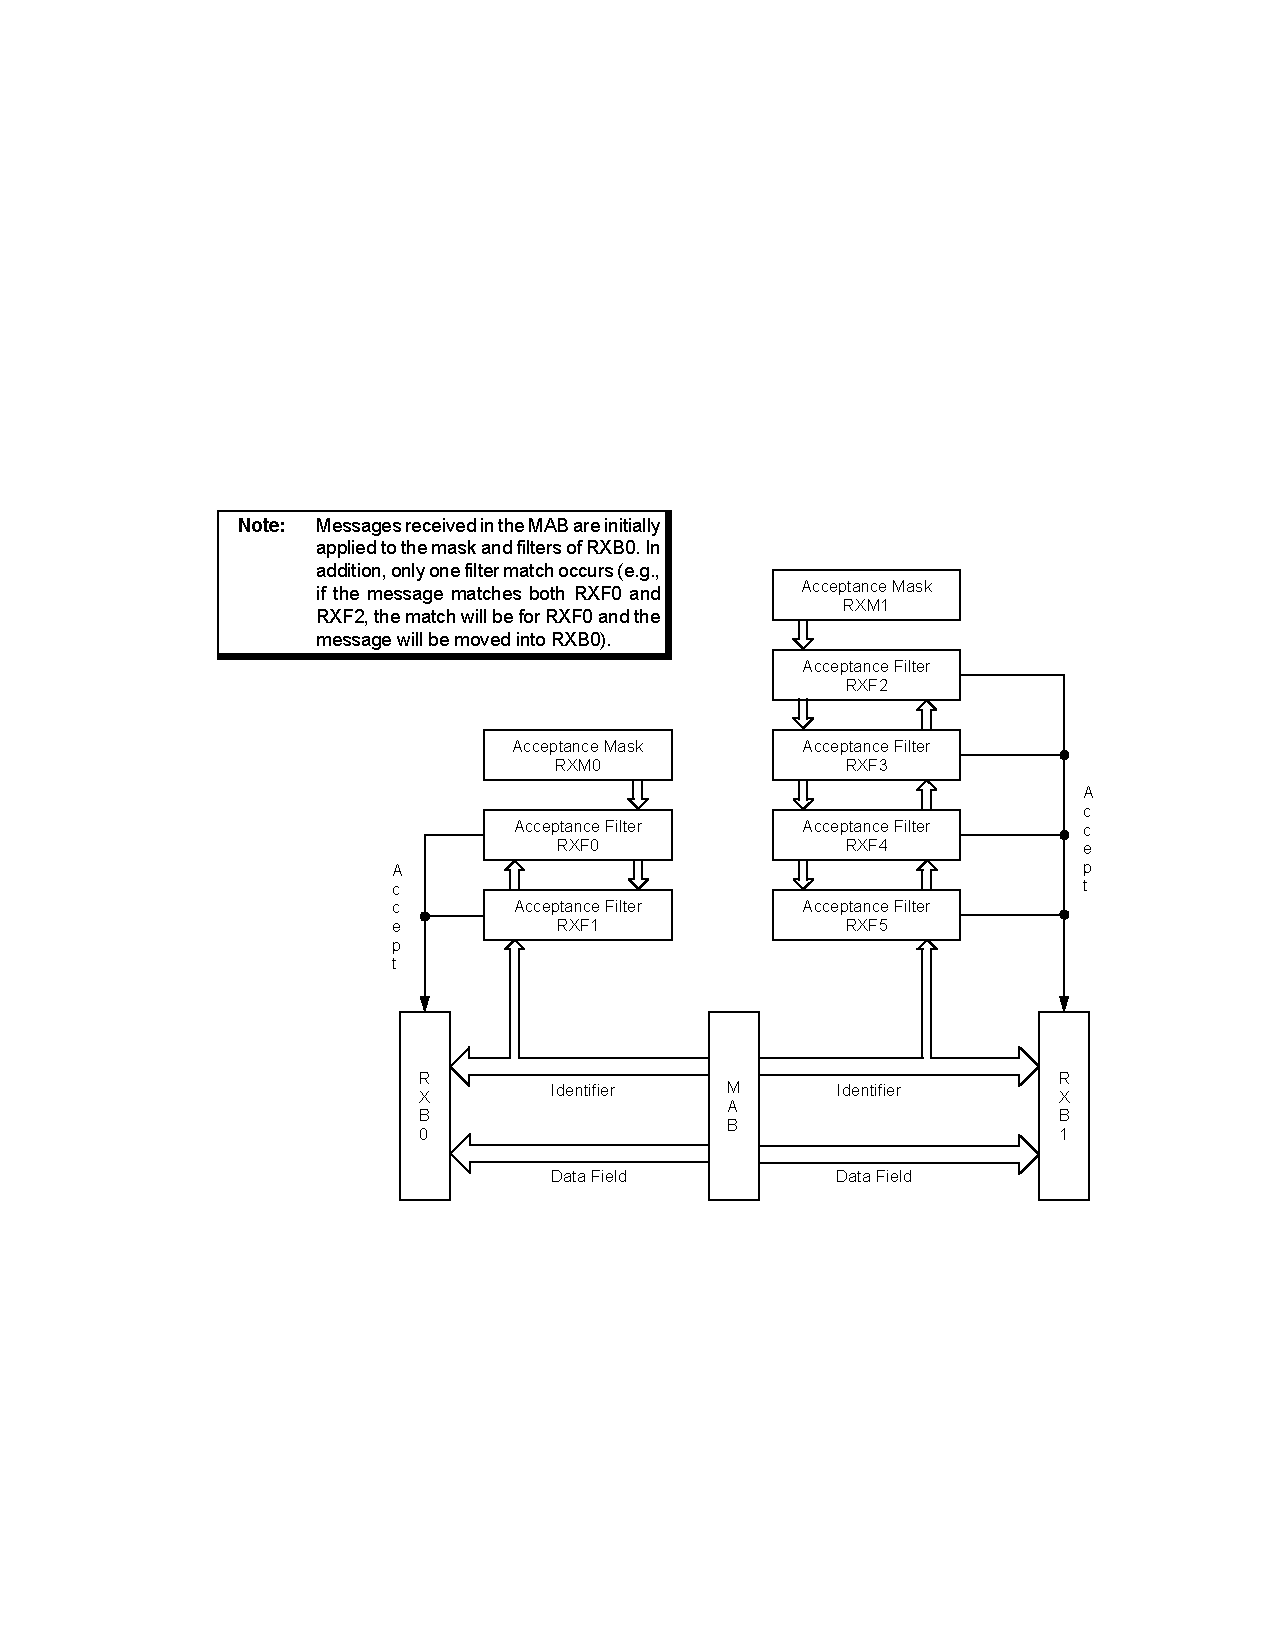
\includegraphics[width=12cm]{mcp2515-filters.pdf}
  \caption{\texttt{MCP2515} acceptance filters}
  \labelFigure{figureFiltres2515}
\end{figure}








\subsection{Primary filter example}

For defining \emph{primary filters}\footnote{For \emph{secondary filters}, see \refSectionPage{secondaryFilters}.}, you write:
{ \small\begin{lstlisting}[language=c++]
void setup () {
  ACAN2515Settings settings (QUARTZ_FREQUENCY, 125 * 1000) ;
  ...
  const ACANPrimaryFilter primaryFilters [] = {
    ACANPrimaryFilter (kData, kExtended, 0x123456), // Filter #0
    ACANPrimaryFilter (kData, kStandard, 0x234),    // Filter #1
    ACANPrimaryFilter (kRemote, kStandard, 0x542)   // Filter #2
  } ;
  const uint32_t errorCode = can.begin (settings,
                                               primaryFilters, // The filter array
                                               3) ; // Filter array size
  ...
}

void loop () {
  CANMessage message ;
  if (can.receive (message)) { // Only frames that pass a filter are retrieved
    if (!message.rtr && message.ext && (message.id == 0x123456)) {
      handle_myMessage_0 (message) ; // Extended data frame, id is 0x123456
    }else if (!message.rtr && !message.ext && (message.id == 0x234)) {
      handle_myMessage_1 (message) ;  // Standard data frame, id is 0x234
    }else if (message.rtr && !message.ext && (message.id == 0x542)) {
      handle_myMessage_2 (message) ;  // Standard remote frame, id is 0x542
    }
  }
  ...
}
\end{lstlisting}}

Each element of the \texttt{primaryFilters} constant array defines an acceptance filter. Should be specified\footnote{There is a fourth optional argument, that is \texttt{NULL} by default -- see \refSectionPage{UsingDispatchMethod}.}:
\begin{itemize}
  \item the required kind: data frames (\texttt{kData}) or remote frames (\texttt{kRemote});
  \item the required format: standard frames (\texttt{kStandard}) or extended frames (\texttt{kExtended});
  \item the required identifier value.
\end{itemize}


{\bf Maximum number of \emph{primary filters}.} The number of \emph{primary filters} is limited: 12 by default, as the default value of \texttt{settings.mConfiguration} is \texttt{ACAN2515Settings::k12\_12\_Filters}. See \refSectionPage{FlexCANconfiguration} for getting the number of \emph{primary filters} for each configuration, and for setting your own configuration.

{\bf Test order.} The \texttt{MCP2515} hardware examines the filters in the increasing order of their indexes in the \texttt{primaryFilters} constant array. As soon as a match occurs, the message is transfered to Rx FIFO buffer and the examination process is completed. If no match occurs, the message is lost.

A consequence is if a filter appears twice, the second occurrence will never match. In the next example, the Filter \#3 will never match, as it is identical to filter \#1.

{ \small\begin{lstlisting}[language=c++]
void setup () {
  ...
  const ACANPrimaryFilter primaryFilters [] = {
    ACANPrimaryFilter (kData, kExtended, 0x123456), // Filter #0
    ACANPrimaryFilter (kData, kStandard, 0x234),    // Filter #1
    ACANPrimaryFilter (kRemote, kStandard, 0x542),  // Filter #2
    ACANPrimaryFilter (kData, kStandard, 0x234)     // Filter #3
  } ;
  ...
}
\end{lstlisting}}



\subsectionLabel{Primary filter as pass-all filter}{passAllPrimaryFilter}

You can specify a primary filter that matches any frame: 
{ \small\begin{lstlisting}[language=c++]
    ACANPrimaryFilter ()
\end{lstlisting}}

You can use it for accepting all frames that did not match previous filters:
{ \small\begin{lstlisting}[language=c++]
void setup () {
  ...
  const ACANPrimaryFilter primaryFilters [] = {
    ACANPrimaryFilter (kData, kExtended, 0x123456), // Filter #0
    ACANPrimaryFilter (kData, kStandard, 0x234),    // Filter #1
    ACANPrimaryFilter (kRemote, kStandard, 0x542),  // Filter #2
    ACANPrimaryFilter ()                            // Filter #3
  } ; // Filter #3 catches any message that did not match filters #0, #1 and #2
  ...
}
\end{lstlisting}}

Be aware if the pass-all filter is not the last one, following ones will never match.
{ \small\begin{lstlisting}[language=c++]
void setup () {
  ...
  const ACANPrimaryFilter primaryFilters [] = {
    ACANPrimaryFilter (kData, kExtended, 0x123456), // Filter #0
    ACANPrimaryFilter (kData, kStandard, 0x234),    // Filter #1
    ACANPrimaryFilter (),                           // Filter #2
    ACANPrimaryFilter (kRemote, kStandard, 0x542)   // Filter #3
  } ; // Filter #3 will never match
  ...
}
\end{lstlisting}}



\subsectionLabel{Primary filter for matching several identifiers}{primaryMultipleFilter}

A primary filter can be configured for matching several identifiers\footnote{A \emph{secondary filter} cannot be configured for matching several identifiers.}. You provide two values: a \texttt{filter\_mask} and a \texttt{filter\_acceptance}. A message with an \texttt{identifier} is accepted if:

\begin{equation*}
  \texttt{filter\_mask}~\&~\texttt{identifier} = \texttt{filter\_acceptance}
\end{equation*}

The $\&$ operator is the bit-wise \emph{and} operator.

Let's take an example: the filter should match standard data frames with identifiers equal to \texttt{0x540}, \texttt{0x541}, \texttt{0x542} and \texttt{0x543}. The four identifiers differs by the two lower bits. As a standard identifiers are 11-bits wide, the \texttt{filter\_mask} is \texttt{0x7FC}. The filter acceptance is \texttt{0x540}. The filter is declared by:

{ \small\begin{lstlisting}[language=c++]
    ...
    ACANPrimaryFilter (kData,     // Accept only data frames
                       kStandard, // Accept only standard frames
                       0x7FC,     // Filter mask
                       0x540)     // Filter acceptance
    ...
}
\end{lstlisting}}

For a standard frame (11-bit identifier), both \texttt{filter\_mask} and a \texttt{filter\_acceptance} should be lower or equal to \texttt{0x7FF}.

For a extended frame (29-bit identifier), both \texttt{filter\_mask} and a \texttt{filter\_acceptance} should be lower or equal to \texttt{0x1FFF\_FFFF}.

Be aware that the \texttt{filter\_mask} and a \texttt{filter\_acceptance} must also conform to the following constraint: if a bit is clear in the \texttt{filter\_mask}, the corresponding bit of the \texttt{filter\_acceptance} should also be clear. In other words, \texttt{filter\_mask} and a \texttt{filter\_acceptance} should check:
\begin{equation*}
  \texttt{filter\_mask}~\&~\texttt{filter\_acceptance} = \texttt{filter\_acceptance}
\end{equation*}

For example, the filter mask \texttt{0x7FC} and the filter acceptance \texttt{0x541} do not conform because the bit 0 of \texttt{filter\_mask} is clear and the bit 0 of the filter acceptance is set.

{\bf A non conform filter may never match.}




\subsectionLabel{Primary filter conformance}{primaryFilterConformance}

The pass-all primary filter (\refSubsectionPage{passAllPrimaryFilter}) always conforms.

For a primary filter for matching several identifiers, see \refSubsectionPage{primaryMultipleFilter}.

For a primary filter for one single identifier:
\begin{itemize}
  \item for a standard frame (11-bit identifier), the given identifier value should be lower or equal to \texttt{0x7FF};
  \item for a extended frame (29-bit identifier), the given identifier value should be lower or equal to \texttt{0x1FFF\_FFFF}.
\end{itemize}

If one or more primary filters do not conform, the execution of the \texttt{begin} method returns an error -- see \refTableauPage{beginErrorCode}.


\subsectionLabel{The \texttt{receive} method revisited}{usingIDXvalue}

The \texttt{receive} method retrieves a received message. When you define primary filters, the value of the \texttt{idx} property of the \texttt{message} is the matching filter index. For example:

{ \small\begin{lstlisting}[language=c++]
void setup () {
  ACAN2515Settings settings (QUARTZ_FREQUENCY, 125 * 1000) ;
  ...
  const ACANPrimaryFilter primaryFilters [] = {
    ACANPrimaryFilter (kData, kExtended, 0x123456), // Filter #0
    ACANPrimaryFilter (kData, kStandard, 0x234),    // Filter #1
    ACANPrimaryFilter (kRemote, kStandard, 0x542)   // Filter #2
  } ;
  const uint32_t errorCode = can.begin (settings, primaryFilters, 3) ;
  ...
}

void loop () {
  CANMessage message ;
  if (can.receive (message)) { // Only frames that pass a filter are retrieved
    switch (message.idx) {
    case 0:
      handle_myMessage_0 (message) ; // Extended data frame, id is 0x123456
      break ;
    case 1:
      handle_myMessage_1 (message) ;  // Standard data frame, id is 0x234
      break ;
    case 2:
      handle_myMessage_2 (message) ;  // Standard remote frame, id is 0x542
      break ;
    default:
      break ;
    }
  }
  ...
}
\end{lstlisting}}

An improvement is to use the \texttt{dispatchReceivedMessage} method -- see \refSectionPage{UsingDispatchMethod}.











\sectionLabel{Secondary filters}{secondaryFilters}

Depending from the configuration, you can define several \emph{secondary filters} -- see \refTableauPage{configFlexCAN}.

% By default, the \texttt{settings.mConfiguration} value is \texttt{k12\_12\_Filters}, allowing up to 12 secondary filters.

%\emph{Secondary filters} are less powerfull than \emph{primary filters} -- a secondary filter cannot match several identifiers. 

\subsection{Secondary filters, without primary filter}

This is an example without primary filter, and with secondary filters:
{ \small\begin{lstlisting}[language=c++]
void setup () {
  ACAN2515Settings settings (QUARTZ_FREQUENCY, 125 * 1000) ;
  ...
  const ACANSecondaryFilter secondaryFilters [] = {
    ACANSecondaryFilter (kData, kExtended, 0x123456), // Filter #0
    ACANSecondaryFilter (kData, kStandard, 0x234),    // Filter #1
    ACANSecondaryFilter (kRemote, kStandard, 0x542)   // Filter #2
  } ;
  const uint32_t errorCode = can.begin (settings,
                                               NULL, 0, // No primary filter
                                               secondaryFilters, // The filter array
                                               3) ; // Filter array size
  ...
void loop () {
  CANMessage message ;
  if (can.receive (message)) { // Only frames that pass a filter are retrieved
    if (!message.rtr && message.ext && (message.id == 0x123456)) {
      handle_myMessage_0 (message) ; // Extended data frame, id is 0x123456
    }else if (!message.rtr && !message.ext && (message.id == 0x234)) {
      handle_myMessage_1 (message) ;  // Standard data frame, id is 0x234
    }else if (message.rtr && !message.ext && (message.id == 0x542)) {
      handle_myMessage_2 (message) ;  // Standard remote frame, id is 0x542
    }
  }
  ...
}
}
\end{lstlisting}}

Each element of the \texttt{secondaryFilters} constant array defines an acceptance filter. Should be specified\footnote{There is a fourth optional argument, that is \texttt{NULL} by default -- see \refSectionPage{UsingDispatchMethod}.}:
\begin{itemize}
  \item the required kind: data frames (\texttt{kData}) or remote frames (\texttt{kRemote});
  \item the required format: standard frames (\texttt{kStandard}) or extended frames (\texttt{kExtended});
  \item the required identifier value.
\end{itemize}

{\bf Maximum number of \emph{secondary filters}.} The number of \emph{secondary filters} is limited: 12 by default, as the default value of \texttt{settings.mConfiguration} is \texttt{ACAN2515Settings::k12\_12\_Filters}. See \refSectionPage{FlexCANconfiguration} for getting the number of \emph{secondary filters} for each configuration, and for changing default value.

{\bf Test order.} The \texttt{MCP2515} hardware examines the filters in the increasing order of their indexes in the \texttt{secondaryFilters} constant array. As soon as a match occurs, the message is transfered to Rx FIFO buffer and the examination process is completed. If no match occurs, the message is lost.

A consequence is if a filter appears twice, the second occurrence will never match.



\subsection{Primary and secondary filters}

This is an example with one primary filter, and two secondary filters:
{ \small\begin{lstlisting}[language=c++]
void setup () {
  ACAN2515Settings settings (QUARTZ_FREQUENCY, 125 * 1000) ;
  ...
  const ACANPrimaryFilter primaryFilters [] = {
    ACANPrimaryFilter (kData, kExtended, 0x123456), // Filter #0
  } ;
  const ACANSecondaryFilter secondaryFilters [] = {
    ACANSecondaryFilter (kData, kStandard, 0x234),    // Filter #1
    ACANSecondaryFilter (kRemote, kStandard, 0x542)   // Filter #2
  } ;
  const uint32_t errorCode = can.begin (settings,
                                               primaryFilters, 
                                               1, // Primary filter array size
                                               secondaryFilters,
                                               2) ; // Secondary filter array size
  ...
void loop () {
  CANMessage message ;
  if (can.receive (message)) { // Only frames that pass a filter are retrieved
    if (!message.rtr && message.ext && (message.id == 0x123456)) {
      handle_myMessage_0 (message) ; // Extended data frame, id is 0x123456
    }else if (!message.rtr && !message.ext && (message.id == 0x234)) {
      handle_myMessage_1 (message) ;  // Standard data frame, id is 0x234
    }else if (message.rtr && !message.ext && (message.id == 0x542)) {
      handle_myMessage_2 (message) ;  // Standard remote frame, id is 0x542
    }
  }
  ...
}
\end{lstlisting}}


{\bf Test order.} The \texttt{MCP2515} hardware performs sequentially:
\begin{itemize}
  \item testing the primary filters in the increasing order of their indexes in the \texttt{primaryFilters} constant array;
  \item as soon as a match with a primary filter occurs, the message is transfered to Rx FIFO buffer and the examination process is completed;
  \item if no match occurs, testing the secondary filters in the increasing order of their indexes in the \texttt{secondaryFilters} constant array;
  \item as soon as a match with a secondary filter occurs, the message is transfered to Rx FIFO buffer and the examination process is completed;
  \item if no match occurs, the message is lost.
\end{itemize}

A consequence is if a filter appears twice, the second occurrence will never match. If a secondary filter matches the same message that a primary filter, the secondary filter will never match.


\subsectionLabel{Secondary filter as pass-all filter}{passAllSecondaryFilter}

You can specify a secondary filter that matches any frame: 
{ \small\begin{lstlisting}[language=c++]
    ACANSecondaryFilter ()
\end{lstlisting}}

You can use it for accepting all frames that did not match previous filters:
{ \small\begin{lstlisting}[language=c++]
void setup () {
  ...
  const ACANSecondaryFilter secondaryFilters [] = {
    ACANSecondaryFilter (kData, kExtended, 0x123456), // Filter #0
    ACANSecondaryFilter (kData, kStandard, 0x234),    // Filter #1
    ACANSecondaryFilter (kRemote, kStandard, 0x542),  // Filter #2
    ACANSecondaryFilter ()                            // Filter #3
  } ; // Filter #3 catches any message that did not match filters #0, #1 and #2
  ...
}
\end{lstlisting}}

Be aware if the pass-all filter is not the last one, following ones will never match.
{ \small\begin{lstlisting}[language=c++]
void setup () {
  ...
  const ACANSecondaryFilter primaryFilters [] = {
    ACANSecondaryFilter (kData, kExtended, 0x123456), // Filter #0
    ACANSecondaryFilter (kData, kStandard, 0x234),    // Filter #1
    ACANSecondaryFilter (),                           // Filter #2
    ACANSecondaryFilter (kRemote, kStandard, 0x542)   // Filter #3
  } ; // Filter #3 will never match
  ...
}
\end{lstlisting}}

If you use a primary pass-all filter, secondary filters will never match:
{ \small\begin{lstlisting}[language=c++]
void setup () {
  ...
  const ACANPrimaryFilter primaryFilters [] = {
    ACANPrimaryFilter (kData, kExtended, 0x123456) // Filter #0
    ACANPrimaryFilter (),                          // Filter #1 - pass-all
  } ;
  const ACANSecondaryFilter secondaryFilters [] = {
    ACANSecondaryFilter (kData, kStandard, 0x234),  // Filter never matches
    ACANSecondaryFilter (kRemote, kStandard, 0x542) // Filter never matches
  } ;
  ...
\end{lstlisting}}



\subsectionLabel{Secondary filter conformance}{secondaryFilterConformance}

The pass-all secondary filter (\refSubsectionPage{passAllSecondaryFilter}) always conforms.

For a standard frame (11-bit identifier), a secondary filter definition is conform if the given identifier value is lower or equal to \texttt{0x7FF}.

For a extended frame (29-bit identifier), a secondary filter definition is conform if the given identifier value is lower or equal to \texttt{0x1FFF\_FFFF}.




\subsectionLabel{The \texttt{receive} method revisited}{usingIDXvalueWithSecondaryFilter}

The \texttt{receive} method retrieves a received message. When you define primary and secondary filters, the value of the \texttt{idx} property of the \texttt{message} is the matching filter index. Filters are numbering from 0, starting by the first element of the first primary filter array until the last one, and continuing from the first element of the secondary filter array, until its last element. So the the \texttt{idx} property  of the \texttt{message} can be used for dispatching the received message:

{ \small\begin{lstlisting}[language=c++]
void setup () {
  ACAN2515Settings settings (QUARTZ_FREQUENCY, 125 * 1000) ;
  ...
  const ACANPrimaryFilter primaryFilters [] = {
    ACANPrimaryFilter (kData, kExtended, 0x123456), // Filter #0
  } ;
  const ACANSecondaryFilter secondaryFilters [] = {
    ACANSecondaryFilter (kData, kStandard, 0x234),    // Filter #1
    ACANSecondaryFilter (kRemote, kStandard, 0x542)   // Filter #2
  } ;
  const uint32_t errorCode = can.begin (settings,
                                               primaryFilters, 1,
                                               secondaryFilters, 2) ;
  ...
}

void loop () {
  CANMessage message ;
  if (can.receive (message)) { // Only frames that pass a filter are retrieved
    switch (message.idx) {
    case 0:
      handle_myMessage_0 (message) ; // Extended data frame, id is 0x123456
      break ;
    case 1:
      handle_myMessage_1 (message) ;  // Standard data frame, id is 0x234
      break ;
    case 2:
      handle_myMessage_2 (message) ;  // Standard remote frame, id is 0x542
      break ;
    default:
      break ;
    }
  }
  ...
}
\end{lstlisting}}

An improvement is to use the \texttt{dispatchReceivedMessage} method -- see \refSectionPage{UsingDispatchMethod}.














\sectionLabel{The \texttt{dispatchReceivedMessage} method}{UsingDispatchMethod}

The last improvement is to call the \texttt{dispatchReceivedMessage} method -- do not call the \texttt{receive} method any more. You can use it if you have defined primary and / or secondary filters that name a call-back function.

The primary and secondary filter constructors have as a last argument a call back function pointer. It defaults to \texttt{NULL}, so until now the code snippets do not  use it.

For enabling the use of the \texttt{dispatchReceivedMessage} method, you add to each filter definition as last argument the function that will handle the message. In the \texttt{loop} function, call the \texttt{dispatchReceivedMessage} method: it dispatches the messages to the call back functions.

{ \small\begin{lstlisting}[language=c++]
void setup () {
  ACAN2515Settings settings (QUARTZ_FREQUENCY, 125 * 1000) ;
  ...
  const ACANPrimaryFilter primaryFilters [] = {
    ACANPrimaryFilter (kData, kExtended, 0x123456, handle_myMessage_0)
  } ;
  const ACANSecondaryFilter secondaryFilters [] = {
    ACANSecondaryFilter (kData, kStandard, 0x234, handle_myMessage_1),
    ACANSecondaryFilter (kRemote, kStandard, 0x542, handle_myMessage_2)
  } ;
  const uint32_t errorCode = can.begin (settings,
                                               primaryFilters, 1,
                                               secondaryFilters, 2) ;
  ...
}

void loop () {
  can.dispatchReceivedMessage () ; // Do not use can.receive any more
  ...
}
\end{lstlisting}}

The \texttt{dispatchReceivedMessage} method handles one message at a time. More precisely:
\begin{itemize}
  \item if it returns \texttt{false}, the driver receive buffer was empty;
  \item if it returns \texttt{true}, the driver receive buffer was not empty, one message has been removed and dispatched.
\end{itemize}

So, the return value can used for emptying and dispatching all received messages:
{ \small\begin{lstlisting}[language=c++]
void loop () {
  while (can.dispatchReceivedMessage ()) {
  }
  ...
}
\end{lstlisting}}

If a filter definition does not name a call back function, the corresponding messages are lost. In the code below, filter \#1 does not name a call back function, standard data frames with identifier \texttt{0x234} are lost.

{ \small\begin{lstlisting}[language=c++]
void setup () {
  ...
  const ACANPrimaryFilter primaryFilters [] = {
    ACANPrimaryFilter (kData, kExtended, 0x123456, handle_myMessage_0)
  } ;
  const ACANSecondaryFilter secondaryFilters [] = {
    ACANSecondaryFilter (kData, kStandard, 0x234), // Filter #1
    ACANSecondaryFilter (kRemote, kStandard, 0x542, handle_myMessage_2)
  } ;
  ...
}
\end{lstlisting}}


The \texttt{dispatchReceivedMessage} method has an optional argument -- \texttt{NULL} by default: a function name. This function is called for every message that pass the receive filters, with an argument equal to the matching filter index:

{ \small\begin{lstlisting}[language=c++]
void filterMatchFunction (const uint32_t inFilterIndex) {
  ...
}

void loop () {
  can.dispatchReceivedMessage (filterMatchFunction) ;
  ...
}
\end{lstlisting}}

You can use this function for maintaining statitistics about receiver filter matches.


\sectionLabel{The \texttt{ACAN::begin} method reference}{beginMethodReference}

\subsection{The \texttt{ACAN::begin} method prototype}

The \texttt{begin} method prototype is:
{ \small\begin{lstlisting}[language=c++]
uint32_t ACAN::begin (const ACAN2515Settings & inSettings,
                      const ACANPrimaryFilter inPrimaryFilters [] = NULL,
                      const uint32_t inPrimaryFilterCount = 0,
                      const ACANSecondaryFilter inSecondaryFilters [] = NULL,
                      const uint32_t inSecondaryFilterCount = 0) ;
\end{lstlisting}}

The four last arguments have default values.

Omitting the last argument makes no secondary filter is defined:
{ \small\begin{lstlisting}[language=c++]
const uint32_t errorCode = can.begin (settings,
                                             primaryFilters, primaryFilterCount,
                                             secondaryFilters) ;
\end{lstlisting}}



Omitting the last two arguments makes no secondary filter is defined:
{ \small\begin{lstlisting}[language=c++]
const uint32_t errorCode = can.begin (settings, primaryFilters, primaryFilterCount) ;
\end{lstlisting}}

Omitting the last three or the last four arguments makes no primary and no secondary filter is defined -- so any (data / remote, standard / extended) frame is received:
{ \small\begin{lstlisting}[language=c++]
const uint32_t errorCode = can.begin (settings, primaryFilters) ;
\end{lstlisting}}

{ \small\begin{lstlisting}[language=c++]
const uint32_t errorCode = can.begin (settings) ;
\end{lstlisting}}





\subsectionLabel{The error code}{errorCodeMethodBegin}

The \texttt{begin} method returns an error code. The value \texttt{0} denotes no error. Otherwise, you consider every bit as an error flag, as described in \refTableau{beginErrorCode}. An error code could report several errors.



\begin{table}[!ht]
  \small
  \onehalfspacing
  \centering
  \begin{tabular}{lllllllllp{6cm}l}
    \multicolumn{9}{c}{\textbf{Error Codes}} & \textbf{Comment} & \textbf{Link}\\
    31 -- 8 & 7 & 6 & 5 & 4 & 3 & 2 & 1 & 0 & & \\
    \texttt{0} ...  \texttt{0} &\texttt{0} &\texttt{0} &\texttt{0} &\texttt{0} &\texttt{0} &\texttt{0} &\texttt{0} &\texttt{0} & No error & \\
    \texttt{0} ...  \texttt{0} &\texttt{0} &\texttt{0} &\texttt{0} &\texttt{0} &\texttt{0} &\texttt{0} &\texttt{0} &\texttt{1} & CAN Bit configuration too far from wished bit rate & \refSubsubsectionPage{CANBitTooFarError}\\
    \texttt{0} ...  \texttt{0} &\texttt{0} &\texttt{0} &\texttt{0} &\texttt{0} &\texttt{0} &\texttt{0} &\texttt{1} &\texttt{0} & Inconsistent CAN Bit configuration & \refSubsubsectionPage{CANBitInconsistentConfigError}\\
    \texttt{0} ...  \texttt{0} &\texttt{x}&\texttt{x} &\texttt{x} &\texttt{x} &\texttt{x} &\texttt{1} &\texttt{0} &\texttt{0} & Too much primary filters & \refSubsubsectionPage{tooMuchPrimaryFiltersError}\\
    \texttt{0} ...  \texttt{0} &\texttt{x} &\texttt{x} &\texttt{x} &\texttt{x} &\texttt{1} &\texttt{x} &\texttt{0} &\texttt{0} & Primary filter conformance error &  \refSubsectionPage{primaryFilterConformanceError}\\
    \texttt{0} ...  \texttt{0} &\texttt{x}&\texttt{x} &\texttt{x} &\texttt{1} &\texttt{x} &\texttt{x} &\texttt{0} &\texttt{0} & Too much secondary filters & \refSubsubsectionPage{tooMuchSecondaryFiltersError}\\
    \texttt{0} ...  \texttt{0} &\texttt{x}&\texttt{x} &\texttt{1} &\texttt{x} &\texttt{x} &\texttt{x} &\texttt{0} &\texttt{0} & Secondary filter conformance error &  \refSubsubsectionPage{secondaryFilterConformanceError}\\
    \texttt{0} ...  \texttt{0} &\texttt{x}&\texttt{1} &\texttt{x} &\texttt{x} &\texttt{x} &\texttt{x} &\texttt{0} &\texttt{0} & \texttt{ACAN::can1} has no Tx alternate pin & \refSubsubsectionPage{noAlternateTxPinError}\\
    \texttt{0} ...  \texttt{0} &\texttt{1}&\texttt{x} &\texttt{x} &\texttt{x} &\texttt{x} &\texttt{x} &\texttt{0} &\texttt{0} & \texttt{ACAN::can1} has no Rx alternate pin & \refSubsubsectionPage{noAlternateRxPinError} \\
  \end{tabular}
  \caption{The \texttt{ACAN::begin} method error codes}
  \labelTableau{beginErrorCode}
\end{table}

The \texttt{ACAN} class defines bit error masks as public static constant properties: 
{ \small\begin{lstlisting}[language=c++]
public: static const uint32_t kCANBitConfigurationTooFarFromWishedBitRate = 1 << 0 ;
public: static const uint32_t kCANBitInconsistentConfiguration            = 1 << 1 ;
public: static const uint32_t kTooMuchPrimaryFilters                      = 1 << 2 ;
public: static const uint32_t kNotConformPrimaryFilter                    = 1 << 3 ;
public: static const uint32_t kTooMuchSecondaryFilters                    = 1 << 4 ;
public: static const uint32_t kNotConformSecondaryFilter                  = 1 << 5 ;
public: static const uint32_t kNoAlternateTxPinForCan1                    = 1 << 6 ;
public: static const uint32_t kNoAlternateRxPinForCan1                    = 1 << 7 ;
\end{lstlisting}}

For example, you can write:
{ \small\begin{lstlisting}[language=c++]
const uint32_t errorCode = can.begin (settings,
                                             primaryFilters, primaryFilterCount,
                                             secondaryFilters, secondaryFilterCount) ;
if (errorCode != 0) {
  // Error(s)
  if (errorCode & ACAN::kTooMuchPrimaryFilters) {
    // Error: too much primary filters
  }
  ...
}
\end{lstlisting}}

\subsubsectionLabel{CAN Bit setting too far from wished rate}{CANBitTooFarError}

This error is raised when the \texttt{mBitConfigurationClosedToWishedRate} of the \texttt{settings} object is false. This means that the \texttt{ACAN2515Settings} constructor cannot compute a CAN bit configuration close enough to the wished bit rate. When the \texttt{begin} is called with \texttt{settings.mBitConfigurationClosedToWishedRate} false, this error is reported. For example:

{ \small\begin{lstlisting}[language=c++]
void setup () {
  ACAN2515Settings settings (QUARTZ_FREQUENCY, 1) ; // 1 bit/s !!!
  // Here, settings.mBitConfigurationClosedToWishedRate is false
  const uint32_t errorCode = can.begin (settings) ;
  // Here, errorCode == ACAN::kCANBitConfigurationTooFarFromWishedBitRateErrorMask
}
\end{lstlisting}}

This error is a fatal error, the driver and the \texttt{MCP2515} module are not configured. See \refSubsectionPage{CANbitSettings} for a discussion about CAN bit setting computation.


\subsubsectionLabel{CAN Bit inconsistent configuration error}{CANBitInconsistentConfigError}

This error is raised when you have changed the CAN bit properties (\texttt{mBitRatePrescaler}, \texttt{mPropagationSegment}, \texttt{mPhaseSegment1}, \texttt{mPhaseSegment2}, \texttt{mRJW}), and one or more resulting values are inconsistent. See \refSubsectionPage{CANBitSettingConsistency}.

%The constraints are:
%\begin{align*}
%1 & \leqslant \texttt{mBitRatePrescaler} \leqslant 256 \\
%1 & \leqslant \texttt{mRJW} \leqslant 4 \\
%1 & \leqslant \texttt{mPropagationSegment} \leqslant 8 \\
%\text{Single sampling: }1 & \leqslant \texttt{mPhaseSegment1} \leqslant 8\\
%\text{Triple sampling: }2 & \leqslant \texttt{mPhaseSegment1} \leqslant 8\\
%2 & \leqslant \texttt{mPhaseSegment2} \leqslant 8 \\
%\texttt{mRJW} &\leqslant \texttt{mPhaseSegment2}
%\end{align*}
%
%Resulting bit rate is given by:
%{\small
%\begin{align*}
%\text{Actual bit rate} & = \frac{16~\text{MHz}}{\texttt{mBitRatePrescaler} \cdot (1 + \texttt{mPropagationSegment} + \texttt{mPhaseSegment1} + \texttt{mPhaseSegment2})}
%\end{align*}
%}
%
%And sampling point (in per-cent unit) are given by:
%{\small
%\begin{align*}
%\text{Sampling point {\it(single sampling)}} & = 100 \cdot \frac{1 + \texttt{mPropagationSegment} + \texttt{mPhaseSegment1}}{1 + \texttt{mPropagationSegment} + \texttt{mPhaseSegment1} + \texttt{mPhaseSegment2}}  \\
%  & \\
%\text{Sampling first point {\it(triple sampling)}} & = 100 \cdot \frac{\texttt{mPropagationSegment} + \texttt{mPhaseSegment1}}{1 + \texttt{mPropagationSegment} + \texttt{mPhaseSegment1} + \texttt{mPhaseSegment2}}
%\end{align*}
%}
%
%does  of the \texttt{settings} object is false. This means that the \texttt{ACAN2515Settings} constructor cannot compute a CAN bit  for the given bit rate. When the \texttt{begin} is called with \texttt{settings.mBitConfigurationClosedToWishedRate} false, this error is reported. For example:
%
%{ \small\begin{lstlisting}[language=c++]
%void setup () {
%  ACAN2515Settings settings (1) ; // 1 bit/s !!!
%  // here, settings.mBitConfigurationClosedToWishedRate is false
%  const uint32_t errorCode = can.begin (settings) ;
%  // here, errorCode is equal to ACAN::kCANBitConfigurationTooFarFromWishedBitRateErrorMask, i.e. 1
%}
%\end{lstlisting}}
%
%This error is a fatal error, the driver and the \texttt{MCP2515} module are not configured. See \refSubsectionPage{CANbitSettings} for a discussion about CAN bit setting computation.




\subsubsectionLabel{Too much primary filters error}{tooMuchPrimaryFiltersError}

The number of \emph{primary filters} is limited. See \refSectionPage{FlexCANconfiguration} for getting the number of \emph{primary filters} for each configuration, and for changing default value.

\subsectionLabel{Primary filters  conformance error}{primaryFilterConformanceError}

One or several primary filters do not conform: see \refSubsectionPage{primaryFilterConformance}. Comment out primary filter definitions until finding the faultly definition.


\subsubsectionLabel{Too much secondary filters error}{tooMuchSecondaryFiltersError}

The number of \emph{secondary filters} is limited. See \refSectionPage{FlexCANconfiguration} for getting the number of \emph{secondary filters} for each configuration, and for changing default value.





\subsubsectionLabel{Secondary filter conformance error}{secondaryFilterConformanceError}

One or several secondary filters do not conform: see \refSubsectionPage{secondaryFilterConformance}. Comment out secondary filter definitions until finding the faultly definition.


\subsubsectionLabel{No alternate Tx pin error}{noAlternateTxPinError}

In the Teensy 3.6, \texttt{ACAN::can1} does not support alternate Tx pin.


\subsubsectionLabel{No alternate Rx pin error}{noAlternateRxPinError}

In the Teensy 3.6, \texttt{ACAN::can1} does not support alternate Rx pin.










\sectionLabel{\texttt{ACAN2515Settings} class reference}{ACAN2515SettingsRef}

{\bf Note. } The \texttt{ACAN2515Settings} class is not Arduino specific. You can compile it on your desktop computer with your favorite C++ compiler. 



\subsectionLabel{The \texttt{ACAN2515Settings} constructor: computation of the CAN bit settings}{CANbitSettings}

The constructor of the \texttt{ACAN2515Settings} has one mandatory argument: the wished bit rate. It tries to compute the CAN bit settings for this bit rate. If it succeeds, the constructed object has its \texttt{mBitConfigurationClosedToWishedRate} property set to \texttt{true}, otherwise it is set to \texttt{false}. For example:
{ \small\begin{lstlisting}[language=c++]
void setup () {
  ACAN2515Settings settings (QUARTZ_FREQUENCY, 1 * 1000 * 1000) ; // 1 Mbit/s
  // Here, settings.mBitConfigurationClosedToWishedRate is true
  ...
}
\end{lstlisting}}

Of course, CAN bit computation always succeeds for classical bit rates: 1 Mbit/s, 500 kbit/s, 250 kbit/s, 125 kbit/s. But CAN bit computation can also succeed for some unusual bit rates, as 842 kbit/s. You can check the result by computing actual bit rate, and the distance from the wished bit rate:
{ \small\begin{lstlisting}[language=c++]
void setup () {
  Serial.begin (9600) ;
  ACAN2515Settings settings (QUARTZ_FREQUENCY, 842 * 1000) ; // 842 kbit/s
  Serial.print ("mBitConfigurationClosedToWishedRate: ") ;
  Serial.println (settings.mBitConfigurationClosedToWishedRate) ; // 1 (--> is true)
  Serial.print ("actual bit rate: ") ;
  Serial.println (settings.actualBitRate ()) ; //  842105 bit/s
  Serial.print ("distance: ") ;
  Serial.println (settings.ppmFromWishedBitRate ()) ; // 124 ppm
  ...
}
\end{lstlisting}}

The actual bit rate is 842,105 bit/s, and its distance from wished bit rate is 124 ppm. "ppm" stands for "part-per-million", and $1~\texttt{ppm} = 10^{-6}$. In other words, $10,000~\texttt{ppm}=1\%$.


By default, a wished bit rate is accepted if the distance from the computed actual bit rate is lower or equal to $1,000~\texttt{ppm} = 0.1~\%$. You can change this default value by adding your own value as second argument of \texttt{ACAN2515Settings} constructor:
{ \small\begin{lstlisting}[language=c++]
void setup () {
  Serial.begin (9600) ;
  ACAN2515Settings settings (QUARTZ_FREQUENCY, 842 * 1000, 100) ; // 842 kbit/s, max distance is 100 ppm
  Serial.print ("mBitConfigurationClosedToWishedRate: ") ;
  Serial.println (settings.mBitConfigurationClosedToWishedRate) ; // 0 (--> is false)
  Serial.print ("actual bit rate: ") ;
  Serial.println (settings.actualBitRate ()) ; //  842105 bit/s
  Serial.print ("distance: ") ;
  Serial.println (settings.ppmFromWishedBitRate ()) ; // 124 ppm
  ...
}
\end{lstlisting}}

The second argument does not change the CAN bit computation, it only changes the acceptance test for setting the \texttt{mBitConfigurationClosedToWishedRate} property. For example, you can specify that you want the computed actual bit to be exactly the wished bit rate:
{ \small\begin{lstlisting}[language=c++]
void setup () {
  Serial.begin (9600) ;
  ACAN2515Settings settings (QUARTZ_FREQUENCY, 500 * 1000, 0) ; // 500 kbit/s, max distance is 0 ppm
  Serial.print ("mBitConfigurationClosedToWishedRate: ") ;
  Serial.println (settings.mBitConfigurationClosedToWishedRate) ; // 1 (--> is true)
  Serial.print ("actual bit rate: ") ;
  Serial.println (settings.actualBitRate ()) ; //  500,000 bit/s
  Serial.print ("distance: ") ;
  Serial.println (settings.ppmFromWishedBitRate ()) ; // 0 ppm
  ...
}
\end{lstlisting}}

The fastest exact bit rate is 3,2 Mbit/s. It works when the \texttt{MCP2515} module is configured in both \emph{loop back} mode (\refSubsubsectionPage{mLoopBackMode}) and \emph{self reception} mode (\refSubsubsectionPage{mSelfReceptionMode}). Note bit rates above 1 Mbit/s do not conform to the \texttt{ISO-11898}; CAN transceivers as \texttt{MCP2551} require the bit rate lower or equal to 1 Mbit/s.


The slowest exact bit rate is 2.5 kbit/s. Note many CAN transceivers as the \texttt{MCP2551} provide "\emph{detection of ground fault (permanent Dominant) on TXD input}". For example, the \texttt{MCP2551} constraints the bit rate to be greater or equal to 16 kbit/s. If you want to work with slower bit rates and you need a transceiver, use one without this detection, as the \texttt{PCA82C250}.


In any way, the bit rate computation always gives a consistent result, resulting an actual bit rate closest from the wished bit rate. For example:
{ \small\begin{lstlisting}[language=c++]
void setup () {
  Serial.begin (9600) ;
  ACAN2515Settings settings (QUARTZ_FREQUENCY, 440 * 1000) ; // 440 kbit/s 
  Serial.print ("mBitConfigurationClosedToWishedRate: ") ;
  Serial.println (settings.mBitConfigurationClosedToWishedRate) ; // 0 (--> is false)
  Serial.print ("actual bit rate: ") ;
  Serial.println (settings.actualBitRate ()) ; //  444,444 bit/s
  Serial.print ("distance: ") ;
  Serial.println (settings.ppmFromWishedBitRate ()) ; // 10,100 ppm
  ...
}
\end{lstlisting}}

You can get the details of the CAN bit decomposition. For example:

{ \small\begin{lstlisting}[language=c++]
void setup () {
  Serial.begin (9600) ;
  ACAN2515Settings settings (QUARTZ_FREQUENCY, 440 * 1000) ; // 440 kbit/s 
  Serial.print ("mBitConfigurationClosedToWishedRate: ") ;
  Serial.println (settings.mBitConfigurationClosedToWishedRate) ; // 0 (--> is false)
  Serial.print ("actual bit rate: ") ;
  Serial.println (settings.actualBitRate ()) ; //  444,444 bit/s
  Serial.print ("distance: ") ;
  Serial.println (settings.ppmFromWishedBitRate ()) ; // 10,100 ppm
  Serial.print ("Bit rate prescaler: ") ;
  Serial.println (settings.mBitRatePrescaler) ; // BRP = 2
  Serial.print ("Propagation segment: ") ;
  Serial.println (settings.mPropagationSegment) ; // PropSeg = 6
  Serial.print ("Phase segment 1: ") ;
  Serial.println (settings.mPhaseSegment1) ; // PS1 = 5
  Serial.print ("Phase segment 2: ") ;
  Serial.println (settings.mPhaseSegment2) ; // PS2 = 6
  Serial.print ("Resynchronization Jump Width: ") ;
  Serial.println (settings.mRJW) ; // RJW = 4
  Serial.print ("Triple Sampling: ") ;
  Serial.println (settings.mTripleSampling) ; // 0, meaning single sampling
  Serial.print ("Sample Point: ") ;
  Serial.println (settings.samplePointFromBitStart ()) ; // 68, meaning 68%
  Serial.print ("Consistency: ") ;
  Serial.println (settings.CANBitSettingConsistency ()) ; // 0, meaning Ok
  ...
}
\end{lstlisting}}

The \texttt{samplePointFromBitStart} method returns sample point, expressed in per-cent of the bit duration from the beginning of the bit.


Note the computation may calculate a bit decomposition too far from the wished bit rate, but it is always consistent. You can check this by calling the \texttt{CANBitSettingConsistency} method.

You can change the property values for adapting to the particularities of your CAN network propagation time. By example, you can increment the \texttt{mPhaseSegment1} value, and decrement the \texttt{mPhaseSegment2} value in order to sample the \texttt{CAN Rx} pin later.

{ \small\begin{lstlisting}[language=c++]
void setup () {
  Serial.begin (9600) ;
  ACAN2515Settings settings (QUARTZ_FREQUENCY, 500 * 1000) ; // 500 kbit/s
  Serial.print ("mBitConfigurationClosedToWishedRate: ") ;
  Serial.println (settings.mBitConfigurationClosedToWishedRate) ; // 1 (--> is true)
  settings.mPhaseSegment1 ++ ; // 5 -> 6: safe, 1 <= PS1 <= 8
  settings.mPhaseSegment2 -- ; // 5 -> 4: safe, 2 <= PS2 <= 8 and RJW <= PS2
  Serial.print ("Sample Point: ") ;
  Serial.println (settings.samplePointFromBitStart ()) ; // 75, meaning 75%
  Serial.print ("actual bit rate: ") ;
  Serial.println (settings.actualBitRate ()) ; //  500000: ok, bit rate did not change
  Serial.print ("Consistency: ") ;
  Serial.println (settings.CANBitSettingConsistency ()) ; // 0, meaning Ok
  ...
}
\end{lstlisting}}

Be aware to always respect CAN bit timing consistency! The constraints are:

\begin{align*}
1 & \leqslant \texttt{mBitRatePrescaler} \leqslant 64 \\
1 & \leqslant \texttt{mSJW} \leqslant 4 \\
1 & \leqslant \texttt{mPropagationSegment} \leqslant 8 \\
\text{Single sampling: }1 & \leqslant \texttt{mPhaseSegment1} \leqslant 8\\
\text{Triple sampling: }2 & \leqslant \texttt{mPhaseSegment1} \leqslant 8\\
2 & \leqslant \texttt{mPhaseSegment2} \leqslant 8 \\
\texttt{mSJW} &<\texttt{mPhaseSegment2}\\
\texttt{mPhaseSegment2} & \leqslant \texttt{mPropagationSegment} + \texttt{mPhaseSegment1}
\end{align*}

Resulting actual bit rate is given by:
{\small
\begin{align*}
\text{Actual bit rate} & = \frac{QuartzFrequency~/~2}{\texttt{mBitRatePrescaler} \cdot (1 + \texttt{mPropagationSegment} + \texttt{mPhaseSegment1} + \texttt{mPhaseSegment2})}
\end{align*}
}

And sampling points (in per-cent unit) are given by:
{\small
\begin{align*}
\text{Sampling point {\it(single sampling)}} & = 100 \cdot \frac{1 + \texttt{mPropagationSegment} + \texttt{mPhaseSegment1}}{1 + \texttt{mPropagationSegment} + \texttt{mPhaseSegment1} + \texttt{mPhaseSegment2}}  \\
  & \\
\text{Sampling first point {\it(triple sampling)}} & = 100 \cdot \frac{\texttt{mPropagationSegment} + \texttt{mPhaseSegment1}}{1 + \texttt{mPropagationSegment} + \texttt{mPhaseSegment1} + \texttt{mPhaseSegment2}}
\end{align*}
}












\subsectionLabel{The \texttt{CANBitSettingConsistency} method}{CANBitSettingConsistency}

This method checks the CAN bit decomposition (given by \texttt{mBitRatePrescaler}, \texttt{mPropagationSegment}, \texttt{mPhaseSegment1}, \texttt{mPhaseSegment2}, \texttt{mRJW} property values) is consistent.

{ \small\begin{lstlisting}[language=c++]
void setup () {
  Serial.begin (9600) ;
  ACAN2515Settings settings (QUARTZ_FREQUENCY, 500 * 1000) ; // 500 kbit/s
  Serial.print ("mBitConfigurationClosedToWishedRate: ") ;
  Serial.println (settings.mBitConfigurationClosedToWishedRate) ; // 1 (--> is true)
  settings.mPhaseSegment1 = 0 ; // Error, mPhaseSegment1 should be >= 1 (and <= 8)
  Serial.print ("Consistency: 0x") ;
  Serial.println (settings.CANBitSettingConsistency (), HEX) ; // 0x10, meaning error
  ...
}
\end{lstlisting}}

The \texttt{CANBitSettingConsistency} method returns $0$ if CAN bit decomposition is consistent. Otherwise, the returned value is a bit field that can report several errors -- see \refTableau{CANBitSettingConsistencyErrorCode}.

\begin{table}[!ht]
  \newcommand\zero{\texttt{0}}
  \newcommand\X{\texttt{x}}
  \small
  \onehalfspacing
  \centering
  \begin{tabular}{llllllllllllll}
    \multicolumn{12}{c}{\textbf{Error Codes}} & \textbf{Error}\\
    31 -- 11 & 10 & 9 & 8 & 7 & 6 & 5 & 4 & 3 & 2 & 1 & 0 & \\
    \zero~...  \zero &\zero &\zero &\zero &\zero &\zero &\zero &\zero &\zero &\zero &\zero &\zero & No error \\
    \zero~...  \zero &\X &\X &\X &\X &\X &\X &\X &\X &\X &\X &\texttt{1} & \texttt{mBitRatePrescaler} == 0\\
    \zero~...  \zero &\X &\X &\X &\X &\X &\X &\X &\X &\X &\texttt{1}&\X & \texttt{mBitRatePrescaler} > 64\\
    \zero~...  \zero &\X &\X &\X &\X &\X &\X &\X &\X &\texttt{1}&\X &\X & \texttt{mPropagationSegment} == 0\\
    \zero~...  \zero &\X &\X &\X &\X &\X &\X &\X &\texttt{1}&\X &\X &\X & \texttt{mPropagationSegment} > 8\\
    \zero~...  \zero &\X &\X &\X &\X &\X &\X &\texttt{1}&\X &\X &\X &\X & \texttt{mPhaseSegment1} == 0\\
    \zero~...  \zero &\X &\X &\X &\X &\X &\texttt{1}&\X &\X &\X &\X &\X & \texttt{mPhaseSegment1} > 8\\
    \zero~...  \zero &\X &\X &\X &\X &\texttt{1}&\X &\X &\X &\X &\X &\X & \texttt{mPhaseSegment2} == 0\\
    \zero~...  \zero &\X &\X &\X &\texttt{1}&\X &\X &\X &\X &\X &\X &\X & \texttt{mPhaseSegment2} > 8\\
    \zero~...  \zero &\X &\X &\texttt{1}&\X &\X &\X &\X &\X &\X &\X &\X & \texttt{mRJW} == 0\\
    \zero~...  \zero &\X &\texttt{1}&\X &\X &\X &\X &\X &\X &\X &\X &\X & \texttt{mRJW} > 4\\
    \zero~...  \zero &\texttt{1}&\X &\X &\X &\X &\X &\X &\X &\X &\X &\X & \texttt{mRJW} > \texttt{mPhaseSegment2}\\
  \end{tabular}
  \caption{The \texttt{ACAN2515Settings::CANBitSettingConsistency} method error codes}
  \labelTableau{CANBitSettingConsistencyErrorCode}
\end{table}

The \texttt{ACAN2515Settings} class defines static constant properties that can be used as mask error:
{ \small\begin{lstlisting}[language=c++]
public: static const uint32_t kBitRatePrescalerIsZero           = 1 <<  0 ;
public: static const uint32_t kBitRatePrescalerIsGreaterThan256 = 1 <<  1 ;
public: static const uint32_t kPropagationSegmentIsZero         = 1 <<  2 ;
public: static const uint32_t kPropagationSegmentIsGreaterThan8 = 1 <<  3 ;
public: static const uint32_t kPhaseSegment1IsZero              = 1 <<  4 ;
public: static const uint32_t kPhaseSegment1IsGreaterThan8      = 1 <<  5 ;
public: static const uint32_t kPhaseSegment2IsZero              = 1 <<  6 ;
public: static const uint32_t kPhaseSegment2IsGreaterThan8      = 1 <<  7 ;
public: static const uint32_t kRJWIsZero                        = 1 <<  8 ;
public: static const uint32_t kRJWIsGreaterThan4                = 1 <<  9 ;
public: static const uint32_t kRJWIsGreaterThanPhaseSegment2    = 1 << 10 ;
\end{lstlisting}}









\subsectionLabel{The \texttt{actualBitRate} method}{actualBitRate}


The \texttt{actualBitRate} method returns the actual bit computed from \texttt{mBitRatePrescaler}, \texttt{mPropagationSegment}, \texttt{mPhaseSegment1}, \texttt{mPhaseSegment2}, \texttt{mRJW} property values.

{ \small\begin{lstlisting}[language=c++]
void setup () {
  Serial.begin (9600) ;
  ACAN2515Settings settings (QUARTZ_FREQUENCY, 440 * 1000) ; // 440 kbit/s 
  Serial.print ("mBitConfigurationClosedToWishedRate: ") ;
  Serial.println (settings.mBitConfigurationClosedToWishedRate) ; // 0 (--> is false)
  Serial.print ("actual bit rate: ") ;
  Serial.println (settings.actualBitRate ()) ; //  444,444 bit/s
  ...
}
\end{lstlisting}}

{\bf Note. } If CAN bit settings are not consistent (see \refSubsectionPage{CANBitSettingConsistency}), the returned value is irrelevant.











\subsectionLabel{The \texttt{exactBitRate} method}{exactBitRate}


The \texttt{exactBitRate} method returns \texttt{true} if the actual bit rate is equal to the wished bit rate, and \texttt{false} otherwise.

{ \small\begin{lstlisting}[language=c++]
void setup () {
  Serial.begin (9600) ;
  ACAN2515Settings settings (QUARTZ_FREQUENCY, 842 * 1000) ; // 842 kbit/s
  Serial.print ("mBitConfigurationClosedToWishedRate: ") ;
  Serial.println (settings.mBitConfigurationClosedToWishedRate) ; // 1 (--> is true)
  Serial.print ("actual bit rate: ") ;
  Serial.println (settings.actualBitRate ()) ; //  842105 bit/s
  Serial.print ("distance: ") ;
  Serial.println (settings.ppmFromWishedBitRate ()) ; // 124 ppm
  Serial.print ("Exact: ") ;
  Serial.println (settings.exactBitRate ()) ; // 0 (---> false)
  ...
}
\end{lstlisting}}

{\bf Note. } If CAN bit settings are not consistent (see \refSubsectionPage{CANBitSettingConsistency}), the returned value is irrelevant.






\subsectionLabel{The \texttt{ppmFromWishedBitRate} method}{ppmFromWishedBitRate}


The \texttt{ppmFromWishedBitRate} method returns the distance from the actual bit rate to the wished bit rate, expressed in part-per-million (ppm): $1~\texttt{ppm} = 10^{-6}$. In other words, $10,000~\texttt{ppm}=1\%$.

{ \small\begin{lstlisting}[language=c++]
void setup () {
  Serial.begin (9600) ;
  ACAN2515Settings settings (QUARTZ_FREQUENCY, 842 * 1000) ; // 842 kbit/s
  Serial.print ("mBitConfigurationClosedToWishedRate: ") ;
  Serial.println (settings.mBitConfigurationClosedToWishedRate) ; // 1 (--> is true)
  Serial.print ("actual bit rate: ") ;
  Serial.println (settings.actualBitRate ()) ; //  842105 bit/s
  Serial.print ("distance: ") ;
  Serial.println (settings.ppmFromWishedBitRate ()) ; // 124 ppm
  ...
}
\end{lstlisting}}

{\bf Note. } If CAN bit settings are not consistent (see \refSubsectionPage{CANBitSettingConsistency}), the returned value is irrelevant.






\subsectionLabel{The \texttt{samplePointFromBitStart} method}{samplePointFromBitStart}


The \texttt{samplePointFromBitStart} method returns the distance of sample point from the start of the CAN bit, expressed in part-per-cent (ppc): $1~\texttt{ppc} = 1\% = 10^{-2}$. If triple sampling is selected, the returned value is the distance of the first sample point from the start of the CAN bit. It is a good practice to get sample point from 65\% to 80\%.

{ \small\begin{lstlisting}[language=c++]
void setup () {
  Serial.begin (9600) ;
  ACAN2515Settings settings (QUARTZ_FREQUENCY, 500 * 1000) ; // 500 kbit/s
  Serial.print ("mBitConfigurationClosedToWishedRate: ") ;
  Serial.println (settings.mBitConfigurationClosedToWishedRate) ; // 1 (--> is true)
  Serial.print ("Sample point: ") ;
  Serial.println (settings.samplePointFromBitStart ()) ; // 68 --> 68%
  ...
}
\end{lstlisting}}

{\bf Note. } If CAN bit settings are not consistent (see \refSubsectionPage{CANBitSettingConsistency}), the returned value is irrelevant.






\subsectionLabel{Properties of the \texttt{ACAN2515Settings} class}{propertiesACAN2515Settings}

All properties of the \texttt{ACAN2515Settings} class are declared \texttt{public} and are initialized (\refTableau{tablePropertiesACAN2515Settings}). The default values of properties from \texttt{mWhishedBitRate} until \texttt{mTripleSampling} corresponds to a CAN bit rate of 250,000 bit/s.

\begin{table}[!ht]
  \small
  \onehalfspacing
  \centering
  \begin{tabular}{llllll}
    \textbf{Property}& \textbf{Type} & \textbf{Initial value} & \textbf{Comment} \\
    \texttt{mWhishedBitRate} & \texttt{uint32\_t} & \texttt{250,000} & See \refSubsectionPage{CANbitSettings}\\
    \texttt{mBitRatePrescaler} & \texttt{uint16\_t} & \texttt{4} & See \refSubsectionPage{CANbitSettings} \\ % (valid values: $1$ ... $256$)\\
    \texttt{mPropagationSegment} & \texttt{uint8\_t} & \texttt{5} & See \refSubsectionPage{CANbitSettings} \\ %(valid values: $1$ ... $8$)\\
    \texttt{mPhaseSegment1} & \texttt{uint8\_t} & \texttt{5} & See \refSubsectionPage{CANbitSettings}\\ % (valid values: $1$ ... $8$)\\
    \texttt{mPhaseSegment2} & \texttt{uint8\_t} & \texttt{5} & See \refSubsectionPage{CANbitSettings} \\ %(valid values: $2$ ... $8$)\\
    \texttt{mRJW} & \texttt{uint8\_t} & \texttt{4} & See \refSubsectionPage{CANbitSettings} \\ %(valid values: $1$ ... $4$)\\
    \texttt{mTripleSampling} & \texttt{bool} & \texttt{false} & See \refSubsectionPage{CANbitSettings} \\
    \texttt{mBitConfigurationClosedToWishedRate} & \texttt{bool} & \texttt{true} & See \refSubsectionPage{CANbitSettings} \\
    \texttt{mListenOnlyMode} & \texttt{bool} & \texttt{false} & See \refSubsubsectionPage{mListenOnlyMode} \\
    \texttt{mSelfReceptionMode} & \texttt{bool} & \texttt{false} & See \refSubsubsectionPage{mSelfReceptionMode} \\
    \texttt{mLoopBackMode} & \texttt{bool} & \texttt{false} & See \refSubsubsectionPage{mLoopBackMode} \\
    \texttt{mConfiguration} & \texttt{tConfiguration} & \texttt{k12\_12\_Filters} & See \refSectionPage{FlexCANconfiguration} \\
    \texttt{mUseAlternateTxPin} & \texttt{bool} & \texttt{false} & See \refSectionPage{alternatePins} \\
    \texttt{mUseAlternateRxPin} & \texttt{bool} & \texttt{false} & See \refSectionPage{alternatePins} \\
    \texttt{mMessageIRQPriority} & \texttt{uint8\_t} & \texttt{64} & See \refSubsubsectionPage{mMessageIRQPriority}\\
    \texttt{mReceiveBufferSize} & \texttt{uint16\_t} & \texttt{32} & See \refSubsectionPage{driverReceiveBufferSize} \\
    \texttt{mTransmitBufferSize} & \texttt{uint16\_t} & \texttt{16} & See \refSubsectionPage{driverTransmitBufferSize} \\
    \texttt{mTxPinIsOpenCollector} & \texttt{bool} & \texttt{false} & See \refSubsubsectionPage{TxPinIsOpenCollector} \\
    \texttt{mRxPinHasInternalPullUp} & \texttt{bool} & \texttt{false} & See \refSubsubsectionPage{RxPinHasInternalPullUp} \\
   \end{tabular}
  \caption{Properties of the \texttt{ACAN2515Settings} class}
  \labelTableau{tablePropertiesACAN2515Settings}
\end{table}


\subsubsectionLabel{The \texttt{mListenOnlyMode} property}{mListenOnlyMode}

This boolean property corresponds to the \texttt{LOM} bit of the FlexCAN \texttt{CTRL1} control register.



\subsubsectionLabel{The \texttt{mSelfReceptionMode} property}{mSelfReceptionMode}

This boolean property corresponds to the complement of the \texttt{SRXDIS} bit of the FlexCAN \texttt{MCR} control register.



\subsubsectionLabel{The \texttt{mLoopBackMode} property}{mLoopBackMode}

This boolean property corresponds to the \texttt{LBP} bit of the FlexCAN \texttt{CTRL1} control register.





\subsubsectionLabel{The \texttt{mMessageIRQPriority} property}{mMessageIRQPriority}

This property sets the priority of the \emph{CAN message} interrupt. Highest priority is $0$, lowest is $255$.







\subsubsectionLabel{The \texttt{mTxPinIsOpenCollector} property}{TxPinIsOpenCollector}

When the \texttt{mTxPinIsOpenCollector} property is set to \texttt{true}, the \texttt{RECESSIVE} output state puts the \texttt{Tx} pin \texttt{Hi-Z}, instead of driving high. The \texttt{Tx} pin is always driving low in \texttt{DOMINANT} state.

\begin{table}[!ht]
%  \small
  \onehalfspacing
  \centering
  \subfloat[\texttt{mTxPinIsOpenCollector} is \texttt{false} (default)]{
    \begin{tabular}{llllll}
      \textbf{Output state} & \textbf{Tx Pin Output} & \\
      \texttt{DOMINANT} & \texttt{0} & \\
      \texttt{RECESSIVE} & \texttt{1} & \\
    \end{tabular}
  }
  \quad\quad\quad\quad\quad
  \subfloat[\texttt{mTxPinIsOpenCollector} is \texttt{true}]{
    \begin{tabular}{llllll}
      & \textbf{Output state} & \textbf{Tx Pin Output} \\
      & \texttt{DOMINANT} & \texttt{0}\\
      & \texttt{RECESSIVE} & \texttt{Hi-Z}\\
    \end{tabular}
  }
  \caption{\texttt{Tx} pin output, following the \texttt{mTxPinIsOpenCollector} property setting}
  \labelTableau{tableTxPinState}
\end{table}



\subsubsectionLabel{The \texttt{mRxPinHasInternalPullUp} property}{RxPinHasInternalPullUp}

By setting this property, the \texttt{Rx} pin is configured with the internal pullup enabled. This ensures that \texttt{RECESSIVE} values are received if the pin is unconnected.






\sectionLabel{CAN controller state}{canControllerState}

Three methods return the CAN controller state, the receive error counter and the transmit error counter.

\subsection{The \texttt{controllerState} method}

{ \small\begin{lstlisting}[language=c++]
public: tControllerState controllerState (void) const ;
\end{lstlisting}}

This method returns the current state (\emph{error active}, \emph{error passive}, \emph{bus off}) of the CAN controller. The \texttt{tControllerState} type is defined by an enumeration:
{ \small\begin{lstlisting}[language=c++]
typedef enum {kActive, kPassive, kBusOff} tControllerState ;
\end{lstlisting}}


\subsection{The \texttt{receiveErrorCounter} method}

{ \small\begin{lstlisting}[language=c++]
public: uint32_t receiveErrorCounter (void) const ;
\end{lstlisting}}



\subsection{The \texttt{transmitErrorCounter} method}

{ \small\begin{lstlisting}[language=c++]
public: uint32_t transmitErrorCounter (void) const ;
\end{lstlisting}}

As the \texttt{CANx\_ESR} FlexCAN control register does not return a valid value when the CAN controller is in the \emph{bus off} state, the value $256$ is forced.







%\sectionLabel{Some CAN networks}{someCANnetworks}
%
%
%\subsection{A typical configuration}
%
%\newcommand\controleurCAN {
%  \draw[thick, fill=white] (0.4, 2.5) -- ++ (0, -1.5) -- ++ (2.2, 0) -- ++ (0, 1.5);
%  \draw (1, 1) node [above] {\footnotesize\tt CANTX};
%  \draw (2, 1) node [above] {\footnotesize\tt CANRX};
%  \draw (1.5, 2.25) node {\footnotesize\it Teensy 3.x};
%}
%
%\newcommand\PMPoint[2] {
%  \draw (#1, #2)[fill=black] circle (.05);
%}
%
%\newcommand\transceiver{
%  \draw (1, 1) [->] -- ++ (0, -1) ;
%  \draw (2, 1) [<-] -- ++ (0, -1) ;
%  \draw (1, -4) -- ++ (0, 1.9) ;
%  \draw (2, -2) -- ++ (0, -1) ;
%  \draw (1, -2.05)[thick, fill=white] circle (0.05) ;
%  \draw[thick, fill=white] (0.4, -2) rectangle ++ (2.2, 2);
%  \draw (1, -2) node [above] {\footnotesize\tt CAN\_L};
%  \draw (2, -2) node [above] {\footnotesize\tt CAN\_H};
%  \draw (1, 0) node [below] {\footnotesize\tt TxD};
%  \draw (2, 0) node [below] {\footnotesize\tt RxD};
%  \draw (1.5, -1) node {\footnotesize\it CAN transceiver};
%  \PMPoint{1}{-4}
%  \PMPoint{2}{-3}
%}
%
%\newcommand\board{
%  \draw[very thick, fill=gray!12] (0, 2.5) -- ++ (0, -5) -- ++ (3, 0) -- ++ (0, 5);
%}
%
%
%\begin{figure}[!ht]
%  \centering
%  \begin{tikzpicture}[line cap=round, line join=round, >=stealth]
%%   \draw (-.5, -4.5) [decorate, decoration=bumps] rectangle ++ (13.5, 5) ;
%   \board
%   \controleurCAN
%   \transceiver
%   \begin{scope}[xshift=5cm]
%     \board
%     \controleurCAN
%     \transceiver
%   \end{scope}
%   \begin{scope}[xshift=10cm]
%     \board
%     \controleurCAN
%     \transceiver
%   \end{scope}
%
%   \draw (12.5, -4) -- ++ (0, 1);
%   \draw (0.5, -4) -- ++ (0, 1);
%
%   \draw (0.5, -4) -- ++ (3, 0);
%   \draw[dotted] (3.5, -4) -- ++ (1, 0);
%   \draw (4.5, -4) -- ++ (3, 0);
%   \draw[dotted] (7.5, -4) -- ++ (1, 0);
%   \draw (8.5, -4) -- ++ (4, 0);
%
%   \draw (0.5, -3) -- ++ (3, 0);
%   \draw[dotted] (3.5, -3) -- ++ (1, 0);
%   \draw (4.5, -3) -- ++ (3, 0);
%   \draw[dotted] (7.5, -3) -- ++ (1, 0);
%   \draw (8.5, -3) -- ++ (4, 0);
%
%   \draw (0.5-.125, -3.75)[fill=white] rectangle ++ (.25, .5) ;
%   \draw (12.5-.125, -3.75)[fill=white] rectangle ++ (.25, .5) ;
%   \draw (0.5, -3.5) node[left] {\footnotesize$120\Omega~$} ;
%   \draw (12.5, -3.5) node[left] {\footnotesize$120\Omega~$} ;
%%   \draw (3, -3) node[above] {\footnotesize\tt CAN\_H} ;
%%   \draw (3, -4) node[above] {\footnotesize\tt CAN\_L} ;
%  \end{tikzpicture}
%  \caption{Schematic diagram of a CAN bus}
%  \labelFigure{figureConnexionTransmetteurRecepteur}
%\end{figure}


%\subsection{Transceivers}
%
%\subsubsection{\texttt{MCP2551}}
%
%The \refFigure{}{connexionMCP2551} shows how to connect a Teensy 3.x to a \texttt{MCP2551} transceiver\footnote{\url{http://ww1.microchip.com/downloads/en/DeviceDoc/20001667G.pdf}}. Note Microchip does not recommend the \texttt{MCP2551} for new design, use the \texttt{MCP2561}\footnote{\url{http://ww1.microchip.com/downloads/en/DeviceDoc/20005167C.pdf}} instead (see \refSubsubsectionPage{MCP2561}).
%
%The \texttt{MCP2551} requires a \texttt{+5V} power supply. The \texttt{CANTX} pin of the Tennsy 3.x can be directly connected to the \texttt{TXD} pin of the \texttt{MCP2551}. As the \texttt{MCP2551} is powered by \texttt{+5V}, the \texttt{RXD} high level can be directly connected to the \texttt{CANRX} pin only for Teensy 3.x that are \texttt{+5V} tolerant, i.e. Teensy 3.1, Teensy 3.2 and Teensy 3.5. {\bf\color{red} Do not connect directly \texttt{RXD} pin to a Teensy 3.6 \texttt{CANRX} pin!} Teensy 3.6 is not \texttt{+5V} tolerant. For Teensy 3.6, you should lower the high level voltage under $3.3~V$, for example by using a resistor bridge that lowers the high level voltage to $\frac{18~k\Omega}{18~k\Omega + 12~k\Omega}\cdot 5~V = 3~V$.
%
%The \texttt{RS} pin is connected to ground: \emph{High-Speed mode is selected by connecting the RS pin to VSS. In this mode, the transmitter output drivers have fast output rise and fall times to support high-speed CAN bus rates}.
%
%The \texttt{VREF} pin is \emph{Reference Voltage Output (defined as VDD/2)}, and is left open.
%
%
%\newcommand\masse[2] {
%  \draw[thick] (#1 -0.2, #2) -- ++ (0.4, 0);
%  \draw[thick] (#1 -0.1, #2-0.1) -- ++ (0.2, 0);
%  \draw[thick] (#1, #2-0.2) -- ++ (0, 0);
%}
%
%\newcommand\MCPvingtCinqCinquanteEtUn[2]{
%  \draw (1, -2.5) -- ++ (0, 0.4) ;
%  \draw (2, -2) -- ++ (0, -0.5) ;
%  \draw (2.6, -1.4) -- ++ (1.4, 0) ;
%  \PMPoint{4}{-1.4}
%  \draw (0.4, -0.6) -- ++ (-0.5, 0) ;
%  \draw (0.4, -1.4) -- ++ (-0.5, 0) -- ++ (0, -0.35) ;
%  \masse{-0.1}{-1.75}
%  \draw (1, -2.05)[thick, fill=white] circle (0.05) ;
%  \draw[thick, fill=white] (0.4, -2) rectangle ++ (2.2, 2);
%  \draw (1, -2) node [above] {\footnotesize\tt CANL};
%  \draw (2, -2) node [above] {\footnotesize\tt CANH};
%  \draw (1, 0) node [below] {\footnotesize\tt TXD};
%  \draw (2, 0) node [below] {\footnotesize\tt RXD};
%  \draw (0.4, -0.6) node [right] {\footnotesize\tt VDD};
%  \draw (-0.1, -0.6) node [left] {\footnotesize\tt +5V};
%  \draw (0.4, -1.4) node [right] {\footnotesize\tt VSS};
%  \draw (2.6, -0.6) node [left] {\footnotesize\tt #1};
%  \draw (2.6, -1.4) node [left] {\footnotesize\tt RS};
%  \draw (1.5, -1) node {\footnotesize\it #2};
%  \draw (1, 0) node[above left] {\footnotesize\tt 1} ;
%  \draw (2, 0) node[above right] {\footnotesize\tt 4} ;
%  \draw (1, -2) node[below left] {\footnotesize\tt 6} ;
%  \draw (2, -2) node[below right] {\footnotesize\tt 7} ;
%  \draw (2.6, -0.6) node[above right] {\footnotesize\tt 5} ;
%  \draw (2.6, -1.4) node[above right] {\footnotesize\tt 8} ;
%  \draw (0.4, -0.6) node[above left] {\footnotesize\tt 3} ;
%  \draw (0.4, -1.4) node[above left] {\footnotesize\tt 2} ;
%}
%
%\begin{figure}[!ht]
%  \centering
%  \subfloat[Teensy 3.1 / 3.2, 3.5, 3.6]{
%    \begin{tikzpicture}[line cap=round, line join=round, >=stealth]
%      \MCPvingtCinqCinquanteEtUn{VREF}{MCP 2551}
%      \draw (2.6, -0.6) -- ++ (0.5, 0) ;
%      \draw (3.1, -0.6) node [right] {\footnotesize\tt\it nc};
%      \draw (2, 0.5) [<-] -- ++ (0, -0.5) ;
%      \draw (2-0.2, 0.5) rectangle ++ (0.4, 1);
%      \draw (2, 1.5) [->] -- ++ (0, 1.0);
%      \draw (2, 2) -- ++ (2, 0);
%      \draw[fill=white] (2.5, 2-0.2) rectangle ++ (1, 0.4);
%      \draw (3, 2) node {\small$18~k\Omega$};
%      \draw (2, 1) node[rotate=90] {\small$12~k\Omega$};
%      \PMPoint{2}{2}
%      \PMPoint{4}{2}
%  
%      \draw[thick, fill=white] (0.4, 4) -- ++ (0, -1.5) -- ++ (2.2, 0) -- ++ (0, 1.5);
%      \draw (1, 2.5) node [above] {\footnotesize\tt CANTX};
%      \draw (2, 2.5) node [above] {\footnotesize\tt CANRX};
%      \draw (1.5, 3.75) node {\footnotesize\it Teensy 3.x};
%      \draw (1, 2.5) [->] -- ++ (0, -2.5) ;
%      \draw (2.6, 3.25) node [left] {\footnotesize\tt GND};
%      \draw (2.6, 3.25) -- ++ (1.4, 0) -- ++ (0, -5);
%      \masse{4}{-1.75}
%    \end{tikzpicture}
%  }
%  \quad\quad\quad\quad
%  \subfloat[Teensy 3.1 / 3.2, 3.5]{
%    \begin{tikzpicture}[line cap=round, line join=round, >=stealth]
%      \MCPvingtCinqCinquanteEtUn{VREF}{MCP 2551}
%      \draw (3.1, -0.6) node [right] {\footnotesize\tt\it nc};
%      \draw (2.6, -0.6) -- ++ (0.5, 0) ;
%      \draw (2, 2.5) [<-] -- ++ (0, -2.5) ;
%  
%      \draw[thick, fill=white] (0.4, 4) -- ++ (0, -1.5) -- ++ (2.2, 0) -- ++ (0, 1.5);
%      \draw (1, 2.5) node [above] {\footnotesize\tt CANTX};
%      \draw (2, 2.5) node [above] {\footnotesize\tt CANRX};
%      \draw (1.5, 3.85) node {\footnotesize\it Teensy 3.1 / 3.2};
%      \draw (1.5, 3.55) node {\footnotesize\it Teensy 3.5};
%      \draw (1, 2.5) [->] -- ++ (0, -2.5) ;
%      \draw (2.6, 3.25) node [left] {\footnotesize\tt GND};
%      \draw (2.6, 3.25) -- ++ (1.4, 0) -- ++ (0, -5);
%      \masse{4}{-1.75}
%      \draw (2.6, 3.75) node[right] {\footnotesize\color{red} Do not use a Teensy 3.6!};
%      \node[rectangle callout, fill=white, draw, callout relative pointer={(-1.7, 0.6)}] at (4.5, 1.5) {\footnotesize\color{red} Teensy 3.6 inputs are not +5V tolerant!};
%    \end{tikzpicture}
%  }
%  \caption{Connecting a \texttt{MCP2551} to a Teensy 3.x}
%  \labelFigure{connexionMCP2551}
%\end{figure}
%
%
%
%\subsubsectionLabel{\texttt{MCP2561}}{MCP2561}
%
%The pinout of the \texttt{MCP2561} is the same than the \texttt{MCP2551}: the \texttt{VREF} output has been renamed as \texttt{SPLIT} (see \refFigure{}{connexionMCP2561}). {\bf\color{red} Do not connect directly \texttt{RXD} pin to a Teensy 3.6 \texttt{CANRX} pin!}
%
%\begin{figure}[!ht]
%  \centering
%  \subfloat[Teensy 3.1 / 3.2, 3.5, 3.6]{
%    \begin{tikzpicture}[line cap=round, line join=round, >=stealth]
%      \MCPvingtCinqCinquanteEtUn{SPLIT}{MCP 2561}
%      \draw (3.1, -0.6) node [right] {\footnotesize\tt\it nc};
%      \draw (2.6, -0.6) -- ++ (0.5, 0) ;
%      \draw (2, 0.5) [<-] -- ++ (0, -0.5) ;
%      \draw (2-0.2, 0.5) rectangle ++ (0.4, 1);
%      \draw (2, 1.5) [->] -- ++ (0, 1.0);
%      \draw (2, 2) -- ++ (2, 0);
%      \draw[fill=white] (2.5, 2-0.2) rectangle ++ (1, 0.4);
%      \draw (3, 2) node {\small$18~k\Omega$};
%      \draw (2, 1) node[rotate=90] {\small$12~k\Omega$};
%      \PMPoint{2}{2}
%      \PMPoint{4}{2}
%  
%      \draw[thick, fill=white] (0.4, 4) -- ++ (0, -1.5) -- ++ (2.2, 0) -- ++ (0, 1.5);
%      \draw (1, 2.5) node [above] {\footnotesize\tt CANTX};
%      \draw (2, 2.5) node [above] {\footnotesize\tt CANRX};
%      \draw (1.5, 3.75) node {\footnotesize\it Teensy 3.x};
%      \draw (1, 2.5) [->] -- ++ (0, -2.5) ;
%      \draw (2.6, 3.25) node [left] {\footnotesize\tt GND};
%      \draw (2.6, 3.25) -- ++ (1.4, 0) -- ++ (0, -5);
%      \masse{4}{-1.75}
%    \end{tikzpicture}
%  }
%  \quad\quad\quad\quad
%  \subfloat[Teensy 3.1 / 3.2, 3.5]{
%    \begin{tikzpicture}[line cap=round, line join=round, >=stealth]
%      \MCPvingtCinqCinquanteEtUn{SPLIT}{MCP 2561}
%      \draw (3.1, -0.6) node [right] {\footnotesize\tt\it nc};
%      \draw (2.6, -0.6) -- ++ (0.5, 0) ;
%      \draw (2, 2.5) [<-] -- ++ (0, -2.5) ;
%  
%      \draw[thick, fill=white] (0.4, 4) -- ++ (0, -1.5) -- ++ (2.2, 0) -- ++ (0, 1.5);
%      \draw (1, 2.5) node [above] {\footnotesize\tt CANTX};
%      \draw (2, 2.5) node [above] {\footnotesize\tt CANRX};
%      \draw (1.5, 3.85) node {\footnotesize\it Teensy 3.1 / 3.2};
%      \draw (1.5, 3.55) node {\footnotesize\it Teensy 3.5};
%      \draw (1, 2.5) [->] -- ++ (0, -2.5) ;
%      \draw (2.6, 3.25) node [left] {\footnotesize\tt GND};
%      \draw (2.6, 3.25) -- ++ (1.4, 0) -- ++ (0, -5);
%      \masse{4}{-1.75}
%      \draw (2.6, 3.75) node[right] {\footnotesize\color{red} Do not use a Teensy 3.6!};
%      \node[rectangle callout, fill=white, draw, callout relative pointer={(-1.7, 0.6)}] at (4.5, 1.5) {\footnotesize\color{red} Teensy 3.6 inputs are not +5V tolerant!};
%    \end{tikzpicture}
%  }
%  \caption{Connecting a \texttt{MCP2561} to a Teensy 3.x}
%  \labelFigure{connexionMCP2561}
%\end{figure}
%
%\subsubsection{\texttt{MCP2562}}
%
%\begin{figure}[!ht]
%  \centering
%  \begin{tikzpicture}[line cap=round, line join=round, >=stealth]
%    \MCPvingtCinqCinquanteEtUn{VIO}{MCP 2562}
%    \draw (2, 0.5) [<-] -- ++ (0, -0.5) ;
%    \draw (1, 0.5) [->] -- ++ (0, -0.5) ;
%
%    \draw[thick, fill=white] (0.4, 2) -- ++ (0, -1.5) -- ++ (2.2, 0) -- ++ (0, 1.5);
%    \draw (1, 0.5) node [above] {\footnotesize\tt CANTX};
%    \draw (2, 0.5) node [above] {\footnotesize\tt CANRX};
%    \draw (1.5, 1.5) node {\footnotesize\it Teensy 3.x};
%    \draw (2.6, 1.75) node [left] {\footnotesize\tt 3.3V};
%    \draw (2.6, 1.25) node [left] {\footnotesize\tt GND};
%    \draw (2.6, 1.25) -- ++ (1.4, 0) -- ++ (0, -3);
%    \draw (2.6, 1.75) -- ++ (0.7, 0) -- ++ (0, -2.35) -- ++ (-0.7, 0);
%    \masse{4}{-1.75}
%  \end{tikzpicture}
%  \caption{Connecting a \texttt{MCP2562} to a Teensy 3.x}
%  \labelFigure{connexionMCP2562}
%\end{figure}
%
%
%\subsection{Networks with no transceiver}

%-----------------------------------------------------------------------------------------------------------------------*
%   F I N    D U    D O C U M E N T                                                                                     *
%-----------------------------------------------------------------------------------------------------------------------*

\end{document}
